\documentclass[preprint,12pt]{elsarticle}

\usepackage[T1]{fontenc}
\usepackage[utf8]{inputenc}
\usepackage{microtype}
\usepackage{amsmath,amssymb,mathtools}
\usepackage{booktabs,multirow,array,tabularx}
\newcolumntype{Y}{>{\raggedright\arraybackslash}X}
\newcolumntype{C}[1]{>{\centering\arraybackslash}p{#1}}
\usepackage{graphicx}
\usepackage{subcaption}
\usepackage{float}
\usepackage{algorithm}
\usepackage{algpseudocode}
\usepackage{enumitem}
\usepackage{siunitx}
\usepackage{xcolor}
\usepackage{tikz}
\usetikzlibrary{arrows.meta,positioning,fit,shapes.geometric}
\usepackage{url}
\usepackage{xspace}
\usepackage{hyperref}
\hypersetup{colorlinks=true,linkcolor=blue!50!black,citecolor=blue!50!black,urlcolor=blue!50!black}
\graphicspath{{figures/main/}{figures/appendix/}}
\sisetup{detect-all,round-mode=places,round-precision=2}
\setlist[itemize]{leftmargin=*,topsep=3pt,itemsep=2pt}
\setlist[enumerate]{leftmargin=*,topsep=3pt,itemsep=2pt}
\newcommand{\method}{H-CSMO\xspace}
\newcommand{\repTrack}{Representative}
\newcommand{\slaTrack}{SLA-stress}
\newcommand{\good}[1]{\textbf{#1}}

\journal{Future Generation Computer Systems}

\begin{document}
\begin{frontmatter}

\title{H-CSMO: Guarded Multi-Profile Search for Carbon-Efficient and Low-Latency Scheduling in Multi-Region Edge--Cloud Systems}

\author[1]{Khalegh Gorji}
\author[2]{Abbas Mirzaei\corref{cor1}}
\ead{A.mirzaei@iau.ac.ir}
\author[1]{Farsad Zamani}
\author[3]{Ramin Karimi}
\author[4]{Nasser Mikaeilvand}
\cortext[cor1]{Corresponding author}

\address[1]{Department of Computer Engineering, South Tehran Branch, Islamic Azad University, Tehran, Iran}
\address[2]{Department of Computer Engineering, Ardabil Branch, Islamic Azad University, Ardabil, Iran}
\address[3]{Department of Computer Engineering, Shahr-e Qods Branch, Islamic Azad University, Shahr-e Qods, Iran}
\address[4]{Department of Computer Science and Mathematics, Central Tehran Branch, Islamic Azad University, Tehran, Iran}

\begin{abstract}
Multi-region edge--cloud scheduling couples decisions that are often optimized separately: where a task runs, when it starts, which processor state it uses, and whether migration is worthwhile. Time-varying regional carbon intensity complicates this trade-off because an energy-efficient placement can be carbon-intensive, while consolidation or carbon shifting can extend the critical completion tail. Fixed scalarization is therefore brittle across sparse and SLA-stressed workloads. We present H-CSMO, a guarded multi-profile search framework that jointly controls placement, temporal shifting, five-state DVFS, migration, and sleep/wake behavior. H-CSMO constructs energy-, carbon-, hybrid-, and latency-oriented candidate pools, estimates workload pressure to adapt active-pool size, and allocates the objective-call budget to stochastic refinement around structured schedules. A protected critical-tail stage isolates the latest-finishing tasks and generates targeted turbo or fastest-feasible-node repairs instead of globally accelerating the schedule. The balanced output is selected only from feasible candidates satisfying guards on controllable carbon, controllable energy, gross carbon, gross energy, and makespan relative to reference and activation anchors. An external simulator evaluates every method, while two-layer accounting separates scheduler-controllable effects from the fixed infrastructure floor so that background leakage does not mask scheduling decisions. Experiments cover 24 Google- and Alibaba-derived scenarios: 12 frozen representative and 12 controlled SLA-constrained stress cells, against eight equal-budget methods including NSGA-II and PPO. H-CSMO achieves the best representative rank (1.98/8) and highest normalized carbon--energy--makespan hypervolume in all 24 scenarios. Under SLA stress, it ranks second (2.64/8), keeps the best makespan rank, and significantly outperforms ECO-PSO, TM-MOAOA, and PPO on all five metrics after Holm correction.
\end{abstract}

\begin{keyword}
Carbon-aware scheduling \sep edge--cloud computing \sep multi-objective optimization \sep DVFS \sep Pareto search \sep task migration \sep critical-tail scheduling
\end{keyword}

\end{frontmatter}

% ---- BEGIN sections/01_introduction.tex ----
\section{Introduction}
\label{sec:introduction}

Edge--cloud infrastructures increasingly host services whose computation cannot be treated as a single data-center placement problem. Industrial monitoring, interactive analytics, distributed inference, and scientific services combine short response-time requirements with heterogeneous execution sites, changing network paths, and different regional electricity mixes \cite{rahmani2025optimizing,pournazari2025computation,Etheredge2026Pulse}. A scheduler operating across this continuum must decide not only \emph{where} a task runs, but also when it should start, which performance state the selected processor should use, and whether moving task state across regions is worth the transfer cost. These decisions are coupled: a faster site can shorten a critical completion path while consuming more power; a cleaner region can require a network transfer; and temporal deferral can exploit a lower-carbon interval only when the remaining deadline slack is sufficient.

The carbon dimension makes this coupling especially important. Regional grid intensity can change substantially within the lifetime of a workload, so a placement that is energy-efficient is not necessarily carbon-efficient. Carbon-aware execution studies have shown that spatial and temporal flexibility can reduce emissions, but the attainable gain depends on workload slack, resource heterogeneity, and the carbon variation actually exposed to the scheduler \cite{West2026CarbonAwareWorkflows,son2025greenscale,zhai2025forecast}. Recent work has consequently moved from cloud-only energy minimization toward carbon-aware orchestration in the cloud-to-edge continuum, including function-variant offloading, spatio-temporal federated orchestration, and energy-harvesting edge--cloud allocation \cite{calavaro2026functionvariants,alshammaa2026federated,fu2026ehcarbon}. In latency-sensitive systems, however, carbon cannot be optimized independently of deadline feasibility and the power states activated by a placement.

Three technical difficulties dominate this scheduling regime. First, sparse and heavily loaded workloads reward different resource-activation policies. A broad active pool improves headroom under contention but may waste baseline energy when only a few tasks are present. Second, a single scalar objective is brittle when the operating regime changes. Carbon, energy, and completion time can exchange rank across candidate schedules even when all schedules meet their deadlines. Third, migration is neither uniformly harmful nor uniformly beneficial: it can expose a cleaner or faster execution site, but it adds transfer delay, network energy, and transfer-related emissions. These effects become harder to reason about when node sleep/wake transitions and DVFS are available at the same time.

Existing schedulers address parts of this problem through different mechanisms. Carbon-aware methods use forecasts or regional intensity signals to shift computation \cite{zhai2024edge,zhai2025forecast,calavaro2026functionvariants}; Pareto methods preserve several trade-off solutions instead of fixing one weight vector \cite{abraham2025multi,Etheredge2026Pulse}; adaptive metaheuristics alter search behavior as the workload changes \cite{satouf2025metaheuristic,tandon2025novel}; and reinforcement-learning schedulers learn policies from observed system states \cite{shen2025reinforcement,anand2025eadrl,nasir2026relto,sravan2026drl}. These directions are complementary, yet two gaps remain relevant to practical multi-region scheduling. The first is \emph{regime robustness}: a method that is tuned for dense contention can activate too many resources on sparse traces, whereas a conservative energy policy may lengthen the critical tail under SLA pressure. The second is \emph{accounting robustness}: if unavoidable infrastructure leakage is mixed with scheduler-controlled energy, a scheduler can appear insensitive simply because a large fixed floor dominates the reported total.

We address these issues with \method, a guarded multi-profile search framework for joint placement, temporal shifting, and DVFS control. The scheduler begins from a common dynamic-greedy reference and constructs carbon-, energy-, latency-, and hybrid-oriented candidate pools. Pool size is adapted to the workload pressure estimated from arrival windows and fastest feasible execution times. Candidate schedules are then refined under an exact objective-call budget, so the search effort is directly comparable with competing metaheuristics. A protected critical-tail stage examines the latest-finishing tasks and creates narrowly targeted turbo and fastest-feasible-node repairs. Crucially, the balanced output is not selected by unconstrained scalarization. It must satisfy fixed guards on controllable carbon, controllable energy, gross energy, gross carbon, and makespan relative to the common reference, the pre-repair anchor, and a deterministic legacy activation anchor.

A second design choice is the evaluation model. We separate the energy and emissions that can change with scheduling decisions from the infrastructure floor that remains even when nodes are in deep-off leakage. Both quantities are reported. The \emph{scheduler-controllable} layer reveals the effect of placement, timing, DVFS, wake transitions, and migration, while the \emph{gross fixed-horizon} layer preserves the complete facility-level result. This distinction avoids treating background leakage as a scheduling gain and makes the observed trade-offs interpretable across workload scales.

The experimental design is deliberately split into two evidence regimes. Twelve frozen representative scenarios retain the original Google- and Alibaba-derived workloads at 30, 60, and 90 tasks. A separate SLA-constrained track contains 12 controlled stress cells created from four 150-task base scenarios and three predeclared workload seeds. Eight methods receive the same external simulator, decision space, feasibility repair, and per-scenario objective-call budget, including NSGA-II and a PPO-based scheduler. Search seeds are summarized inside each scenario before paired statistical inference, so repeated optimizer seeds are not treated as independent workloads.

The main contributions are as follows:
\begin{itemize}
    \item We formulate a joint edge--cloud scheduling model in which node placement, bounded temporal shifting, five-state DVFS, migration, sleep/wake behavior, and regional carbon intensity are evaluated within one shared decision space.
    \item We develop a workload-adaptive multi-profile search strategy that constructs energy-, carbon-, hybrid-, and latency-oriented active pools and allocates a fixed evaluation budget across deterministic structure and stochastic refinement.
    \item We introduce protected critical-tail repair and guard-based balanced selection, which target the latest-finishing tasks without allowing latency repair to ignore predeclared energy, carbon, and gross-accounting limits.
    \item We introduce transparent two-layer accounting that reports scheduler-controllable energy and emissions separately from the fixed infrastructure floor while retaining gross fixed-horizon values for system-level comparison.
    \item We provide a reproducible evaluation protocol with eight equal-budget methods, workload-level paired statistics, Pareto indicators, ablations, sensitivity analysis, exact search-call accounting, and schedule-level artifact replay.
\end{itemize}

The remainder of the paper is organized as follows. Section~\ref{sec:related} reviews carbon-aware, adaptive, learning-based, and multi-objective schedulers. Section~\ref{sec:model} defines the system and accounting model. Section~\ref{sec:method} presents \method, followed by its algorithmic properties in Section~\ref{sec:properties}. Section~\ref{sec:experimental} describes the traces, baselines, fairness controls, and statistics. Section~\ref{sec:results} reports the results, Section~\ref{sec:discussion} interprets the observed trade-offs, and Section~\ref{sec:conclusion} concludes the paper.
% ---- END sections/01_introduction.tex ----
% ---- BEGIN sections/02_related_work.tex ----
\section{Related Work}
\label{sec:related}

The scheduling problem considered here lies at the intersection of carbon-aware orchestration, multi-objective edge--cloud scheduling, adaptive metaheuristics, and learning-based control. These areas have developed quickly, but they expose different assumptions about workload slack, adaptation cost, and the way competing objectives are represented.

\subsection{Carbon-aware scheduling across the cloud--edge continuum}

Carbon-aware execution first gained traction in geographically distributed systems because the same unit of energy can carry different emissions at different places and times. West et al. quantified the practical potential of carbon-aware execution for scientific workflows and showed that the available flexibility, rather than carbon variation alone, determines the achievable benefit \cite{West2026CarbonAwareWorkflows}. GreenScale by Son et al. extended carbon optimization toward edge computing by considering the interaction between execution location and system carbon cost \cite{son2025greenscale}. Zhai et al. used forecast-driven two-stage scheduling to align geo-distributed workloads with wind availability, emphasizing that temporal prediction can be as important as spatial placement \cite{zhai2025forecast}.

Recent 2026 work has made the carbon model more tightly coupled to continuum orchestration. Calavaro et al. considered carbon-aware offloading with function variants in serverless cloud-to-edge systems, where application variants change the execution trade-off itself \cite{calavaro2026functionvariants}. Al-Shammaa and Al-Hadrawi formulated federated edge--cloud orchestration with dynamic spatio-temporal workload management \cite{alshammaa2026federated}, while Fu et al. studied carbon-aware resource allocation and offloading when edge resources interact with energy harvesting \cite{fu2026ehcarbon}. These studies establish that carbon-aware scheduling is no longer a simple region-selection problem. The remaining difficulty addressed in this paper is narrower but operationally important: carbon decisions are made jointly with sleep/wake transitions, DVFS, migration energy, and a hard latency tail, and the reported carbon benefit is separated from the non-controllable infrastructure floor.

\subsection{Multi-objective and Pareto scheduling}

Multi-objective scheduling avoids reducing heterogeneous operational goals to a single metric. Abraham et al. survey cloud task schedulers that use Pareto or weighted multi-objective formulations and identify makespan, energy, utilization, and cost as recurring objectives \cite{abraham2025multi}. In edge--cloud settings, Etheredge et al. proposed PULSE, a distributed scheduler for service-based applications across multi-cluster cloud--edge--IoT infrastructures \cite{Etheredge2026Pulse}. Younesi et al. considered multi-objective energy optimization in IoT-integrated cyber-physical systems \cite{younesi2025moticps}. These methods motivate preserving trade-off structure rather than presenting a single score as universally optimal.

Several metaheuristic schedulers have also targeted the same metric family. Pournazari et al. proposed energy-centric multi-objective offloading in fog computing \cite{pournazari2025multi}; Khaledian et al. combined TOPSIS with multi-objective Archimedes optimization in TM-MOAOA \cite{khaledian2025tm}; and Tandon et al. used a hybrid metaheuristic to reduce makespan and imbalance in cloud scheduling \cite{tandon2025novel}. The distinction in \method is that the Pareto archive is accompanied by named operating profiles and a guarded final selector. The search can therefore retain diverse candidates while the deployed balanced schedule is prevented from purchasing a latency improvement with an unbounded energy or carbon regression.

\subsection{Adaptive metaheuristic scheduling}

Population-based optimizers remain attractive when the scheduling objective is non-smooth, mixed discrete/continuous, and expensive to differentiate. Satouf et al. studied metaheuristic scheduling for latency-sensitive IoT applications at the edge \cite{satouf2025metaheuristic}; Pinky and Verma combined metaheuristics for delay and energy optimization in cloud--fog systems \cite{pinky2025enhanced}; and Pillai et al. used hybrid metaheuristics for fog-layer resource management \cite{sanjaikanth2025optimizing}. Spider-monkey-based scheduling has also been applied to cloud load balancing and multi-objective task allocation \cite{verma2024load,amer2024efficient,khaleel2025application}.

The common strength of these methods is flexible exploration, but their behavior depends strongly on the candidate representation and on how the search is seeded. A generic mutation operator can spend much of its budget rediscovering obviously poor schedules when the feasible space includes placement, timing, and DVFS simultaneously. \method therefore gives structure to the search before stochastic refinement: node pools are ranked by energy, carbon, speed, and hybrid scores; profile-specific constructors build feasible schedules; and stochastic perturbations are concentrated around these structured candidates. This makes the evaluation budget itself part of the algorithmic design rather than an incidental stopping condition.

\subsection{Learning-based adaptive scheduling}

Deep reinforcement learning provides another route to adaptation by learning a policy over a state/action representation. Shen et al. applied reinforcement learning to task scheduling in heterogeneous end--edge--cloud systems \cite{shen2025reinforcement}; Anand and Karthikeyan proposed EADRL with adaptive exploration for dynamic edge--cloud scheduling \cite{anand2025eadrl}; and Ismail et al. reviewed DQN-, DDQN-, actor--critic-, and related approaches for multi-access edge computing \cite{ismail2025survey}. More recent work focuses directly on multi-objective reward design. RELTO uses PPO with context-aware adaptive reward weighting for reliability-oriented MEC offloading \cite{nasir2026relto}, and Sravan and Shaik formulate a DRL scheduler for latency, energy, and SLA optimization in edge--cloud systems \cite{sravan2026drl}. Federated reinforcement learning has also been used to coordinate adaptive stream scheduling across edge and cloud resources \cite{lajili2026federated}.

Learning-based schedulers can encode long-range state dependencies that hand-designed search operators do not capture. Their practical cost, however, depends on training, reward calibration, and the stability of the deployment distribution. For this reason, the experiments in this paper include an imitation-warm-started PPO scheduler in the same external decision space and with the same simulator-call budget as the classical optimizers. The comparison is therefore about the quality and cost of decision generation under a shared evaluator, rather than about an artificially advantaged simulator interface.

\subsection{Positioning of \method}

Table~\ref{tab:related-positioning} summarizes the closest methodological directions. The contribution of \method is not a new carbon signal or a new isolated optimizer operator. It is the combination of (i) joint placement--time--DVFS decisions, (ii) workload-dependent active-pool construction, (iii) explicit multi-profile search, (iv) critical-tail repair, and (v) protected selection under two-layer energy/carbon accounting. That combination is designed for the case in which the best carbon schedule, the best energy schedule, and the fastest schedule can be different points in the same scenario.

\begin{table*}[t]
\centering
\caption{Positioning of representative scheduling directions relative to the control dimensions used in this study.}
\label{tab:related-positioning}
\scriptsize
\setlength{\tabcolsep}{3pt}
\begin{tabularx}{\textwidth}{p{2.65cm}C{1.0cm}C{1.0cm}C{1.35cm}C{1.35cm}C{1.15cm}Y}
\toprule
Direction & Carbon & Energy & Latency/ SLA & Temporal shift & DVFS & Main distinction relative to \method \\
\midrule
Forecast-driven carbon scheduling \cite{zhai2025forecast,calavaro2026functionvariants} & \checkmark & \checkmark & limited & \checkmark & -- & Strong spatio-temporal carbon control; does not use the guarded multi-profile critical-tail mechanism studied here. \\
Distributed multi-objective scheduling \cite{Etheredge2026Pulse} & context & \checkmark & \checkmark & context & -- & Distributed Pareto/service placement with a different decision representation and power-state model. \\
Adaptive DRL \cite{nasir2026relto,sravan2026drl} & possible & \checkmark & \checkmark & policy dep. & policy dep. & Learns a policy/reward mapping and pays training/inference cost rather than using a bounded profile search. \\
Metaheuristic hybrids \cite{pournazari2025multi,khaledian2025tm,amer2024efficient} & method dep. & \checkmark & \checkmark & limited & method dep. & Flexible search, typically without the same active-pool, two-layer accounting, and protected tail selector. \\
\method & \checkmark & \checkmark & \checkmark & \checkmark & five states & Joint control with equal-budget profile search, two-layer accounting, and protected final selection. \\
\bottomrule
\end{tabularx}
\end{table*}
% ---- END sections/02_related_work.tex ----
% ---- BEGIN sections/03_system_model.tex ----
\section{System Model and Problem Formulation}
\label{sec:model}

\subsection{Infrastructure, workload, and notation}

We consider a set of compute nodes $\mathcal{N}=\{1,\ldots,M\}$ distributed across six geographical regions. Each node $j\in\mathcal{N}$ has a type $\tau_j\in\{\text{edge},\text{regional},\text{cloud}\}$, region $r_j$, CPU and memory capacities $C^{\mathrm{cpu}}_j$ and $C^{\mathrm{mem}}_j$, and an explicit power-state model. The workload is a set $\mathcal{T}=\{1,\ldots,N\}$ of independent tasks. Task $i$ is described by
\begin{equation}
\mathcal{Q}_i=\left(a_i,d_i,w_i,c_i,m_i,v_i,r_i^0,q_i\right),
\end{equation}
where $a_i$ is the arrival time, $d_i$ is the deadline, $w_i$ is observed CPU work, $c_i$ and $m_i$ are requested CPU and memory, $v_i$ is migration state size, $r_i^0$ is the initial region, and $q_i$ is the service class (urgent, standard, or flexible). The Google- and Alibaba-derived scenarios preserve source identifiers so that every scheduled row can be replayed against the original task record.

Each task receives one triplet of control variables,
\begin{equation}
\mathbf{y}_i=\left(j_i,\delta_i,f_i\right),
\label{eq:decision-triplet}
\end{equation}
where $j_i$ is a feasible node, $\delta_i\in[0,1]$ is a temporal-shift fraction, and $f_i\in\mathcal{F}$ is one of five DVFS states. The complete search vector has dimension $3N$. Internally, node and DVFS choices are represented by normalized keys in $[0,1)$ so that every compared optimizer acts on the same continuous vector and the same decoder maps that vector to discrete controls.

\subsection{Execution time, temporal shifting, and resource feasibility}

Let $\xi_{\tau_j}$ denote the baseline speed factor of node type $\tau_j$ and $\sigma_{f_i}$ the speed multiplier of DVFS state $f_i$. The execution time of task $i$ on node $j_i$ is
\begin{equation}
T^{\mathrm{exec}}_i=\frac{w_i}{c_i\,\xi_{\tau_{j_i}}\,\sigma_{f_i}},
\label{eq:runtime}
\end{equation}
with $\xi_{\mathrm{edge}}=0.8$, $\xi_{\mathrm{regional}}=1.0$, and $\xi_{\mathrm{cloud}}=1.25$ in the frozen simulator.

When $r_i^0\neq r_{j_i}$, task state is transferred before execution. Let $B_{uv}$ denote link bandwidth in Gbit/s and $L_{uv}$ the round-trip latency in seconds from region $u$ to $v$. For migration state $v_i$ expressed in GiB, the simulator transfer time is
\begin{equation}
T^{\mathrm{net}}_i=\frac{8v_i}{B_{r_i^0,r_{j_i}}}+L_{r_i^0,r_{j_i}},
\label{eq:transfer-time}
\end{equation}
with zero transfer cost for same-region execution. The earliest possible start is
\begin{equation}
e_i=a_i+T^{\mathrm{net}}_i,
\end{equation}
and the latest target start that leaves one nominal runtime before the deadline is
\begin{equation}
\ell_i=\max\{e_i,d_i-T^{\mathrm{exec}}_i\}.
\end{equation}
The temporal key selects
\begin{equation}
\hat{s}_i=e_i+\delta_i(\ell_i-e_i).
\label{eq:temporal-target}
\end{equation}
The actual start $t_i^{\mathrm{s}}$ is the earliest time no earlier than $\hat{s}_i$ for which concurrent reservations satisfy
\begin{align}
\sum_{k:\,t\in[t_k^{\mathrm{s}},t_k^{\mathrm{f}})} c_k &\le C^{\mathrm{cpu}}_{j_i}, \\
\sum_{k:\,t\in[t_k^{\mathrm{s}},t_k^{\mathrm{f}})} m_k &\le C^{\mathrm{mem}}_{j_i},
\label{eq:resource-capacity}
\end{align}
where $t_i^{\mathrm{f}}=t_i^{\mathrm{s}}+T^{\mathrm{exec}}_i$. If the decoded candidate misses $d_i$, the common evaluator first retries the same node at the performance DVFS state with no temporal shift; if the deadline is still missed, it evaluates all task-feasible nodes under the same repair setting and chooses the earliest feasible completion. This repair is external to every optimizer and therefore does not provide a method-specific advantage.

The workload makespan and deadline statistics are
\begin{align}
T_{\max} &= \max_{i\in\mathcal{T}} t_i^{\mathrm{f}}-\min_{i\in\mathcal{T}} a_i, \\
\mathrm{DMR} &= \frac{1}{N}\sum_{i=1}^{N}\mathbb{I}[t_i^{\mathrm{f}}>d_i], \\
\mathrm{Tard} &= \sum_{i=1}^{N}\max(0,t_i^{\mathrm{f}}-d_i).
\label{eq:latency-metrics}
\end{align}

\subsection{DVFS, sleep/wake, and facility power}

The five DVFS states are $\mathcal{F}=\{$eco-low, eco, balanced, performance, turbo$\}$. State $f$ scales nominal idle and dynamic powers by $\alpha_f^{\mathrm{idle}}$ and $\alpha_f^{\mathrm{dyn}}$. Let $\mathcal{A}_j(t)$ be the tasks executing on node $j$ at time $t$. When $\mathcal{A}_j(t)\neq\varnothing$, the simulator uses
\begin{equation}
P_j^{\mathrm{act}}(t)=\mathrm{PUE}_{r_j}\!\left[
P_j^{\mathrm{idle}}\max_{i\in\mathcal{A}_j(t)}\alpha_{f_i}^{\mathrm{idle}}
+P_j^{\mathrm{dyn}}\sum_{i\in\mathcal{A}_j(t)}
\frac{c_i}{C_j^{\mathrm{cpu}}}\alpha_{f_i}^{\mathrm{dyn}}
\right].
\label{eq:active-power}
\end{equation}
This interval formulation matches the evaluator when tasks with different DVFS states overlap on the same node. Outside active intervals, the node is charged at standby, sleep, or deep-off leakage according to the surrounding reservations and the minimum sleep-time rule. Wake energy is charged whenever a node is first activated or reactivated after a sleep-eligible gap. Predictive wake is available to every scheduler because arrivals are declared by the scenario; therefore wake latency is planned before a reserved start rather than injected as a method-specific deadline penalty.

The migration network consumes $e_{uv}$ Wh per GiB on an inter-region link. Migration energy and its associated emissions are
\begin{align}
E_i^{\mathrm{mig}} &= v_i e_{r_i^0,r_{j_i}}, \\
C_i^{\mathrm{mig}} &= \frac{E_i^{\mathrm{mig}}}{1000}\,\bar{\gamma}_{r_i^0,r_{j_i}}(a_i),
\label{eq:migration-energy}
\end{align}
where $\bar{\gamma}_{uv}$ is the mean source/destination carbon intensity at the task-arrival time used by the frozen evaluator. Carbon intensity $\gamma_r(t)$ is piecewise constant over 30-minute forecast slots in the experiments.

\subsection{Two-layer energy and carbon accounting}
\label{sec:two-layer}

A fixed background floor can mask the effect of a scheduler when workloads differ in duration or density. We therefore report both the gross facility result and the portion above an explicitly declared deep-off floor. The deep-off power of node $j$ is
\begin{equation}
P^{\mathrm{floor}}_j=\rho_{\mathrm{off}}P_j^{\mathrm{idle}}\mathrm{PUE}_{r_j}, \qquad \rho_{\mathrm{off}}=0.01.
\label{eq:floor-power}
\end{equation}
Let $t_0$ be the scenario origin and $t_f=\max_i t_i^{\mathrm{f}}$ the schedule completion time. The finish-bounded gross energy is
\begin{equation}
E^{\mathrm{finish}}_{\mathrm{gross}}
=\sum_{j\in\mathcal{N}}\int_{t_0}^{t_f}P_j(t)\,dt
+\sum_i E_i^{\mathrm{mig}},
\label{eq:finish-energy}
\end{equation}
and the finish-bounded floor is
\begin{equation}
E^{\mathrm{finish}}_{\mathrm{floor}}
=\sum_{j\in\mathcal{N}}P^{\mathrm{floor}}_j(t_f-t_0).
\end{equation}
The scheduler-controllable increment is then
\begin{equation}
E_{\mathrm{ctrl}}=\max\left(0,E^{\mathrm{finish}}_{\mathrm{gross}}-E^{\mathrm{finish}}_{\mathrm{floor}}\right).
\label{eq:controllable-energy}
\end{equation}
For gross comparison, the evaluator extends each schedule to the common horizon
\begin{equation}
H=\max\{t_f,\max_i d_i,\max_i a_i\},
\label{eq:fixed-horizon}
\end{equation}
which is identical across feasible schedules for the same scenario. The fixed-horizon gross energy is
\begin{equation}
E_{\mathrm{gross}}=E^{\mathrm{finish}}_{\mathrm{gross}}+
\sum_j P^{\mathrm{floor}}_j\max(0,H-t_f).
\label{eq:gross-energy}
\end{equation}

Emissions are integrated over the same power intervals using the region-specific carbon process. Denoting this integration operator by $\Gamma[\cdot]$, we report
\begin{align}
C_{\mathrm{ctrl}} &= \max\left(0,C^{\mathrm{finish}}_{\mathrm{gross}}-C^{\mathrm{finish}}_{\mathrm{floor}}\right), \\
C_{\mathrm{gross}} &= C^{\mathrm{finish}}_{\mathrm{gross}}+C^{\mathrm{post}}_{\mathrm{floor}}.
\label{eq:carbon-layers}
\end{align}
The gross quantities are never relabeled as controllable savings; both layers appear in the results.

\subsection{Optimization target}

The scheduling problem is not reduced to one universal scalar. Its primary objective vector is
\begin{equation}
\mathbf{g}(\mathbf{y})=
\left(C_{\mathrm{ctrl}},E_{\mathrm{ctrl}},C_{\mathrm{gross}},E_{\mathrm{gross}},T_{\max},V_{\mathrm{mig}}\right),
\label{eq:objective-vector}
\end{equation}
subject to the resource constraints in Eq.~\eqref{eq:resource-capacity} and deadline feasibility in Eq.~\eqref{eq:latency-metrics}. $V_{\mathrm{mig}}=\sum_i v_i\mathbb{I}[r_i^0\neq r_{j_i}]$ is reported together with migration energy and emissions. The algorithm maintains several profile-specific scalar utilities only to guide search and final operating-point selection; Pareto dominance is computed directly from the physical metrics in Eq.~\eqref{eq:objective-vector}.
% ---- END sections/03_system_model.tex ----
% ---- BEGIN sections/04_method.tex ----
\section{H-CSMO: Guarded Multi-Profile Search}
\label{sec:method}

\subsection{Design overview}

\method operates on the shared $3N$-dimensional representation in Eq.~\eqref{eq:decision-triplet}. Its search is organized around four operating profiles rather than one fixed scalarization: balanced, carbon, energy, and latency-guarded profiles. Each profile changes three things together: the node-ranking criterion used to construct active pools, the admissible DVFS/time-shift options, and the utility used to rank candidate schedules. The balanced profile is the reported default operating point; the other profiles populate the archive and expose alternative carbon, energy, and latency trade-offs.

Figure~\ref{fig:workflow} shows the control flow. The shared simulator first evaluates a dynamic-greedy anchor. Structured constructors then generate profile-specific candidates from ranked node pools. A workload-pressure estimator changes the number of active nodes used by the representative-regime constructors. The remaining objective-call budget is spent on grouped stochastic perturbations around structured leaders and on diversification around the common anchor. The final phase creates targeted repairs for the tasks that finish last, filters all feasible candidates through fixed protection rules, and returns the fastest protected balanced candidate. The non-dominated records remain available for Pareto analysis.

\begin{figure*}[t]
\centering
\resizebox{0.98\textwidth}{!}{%
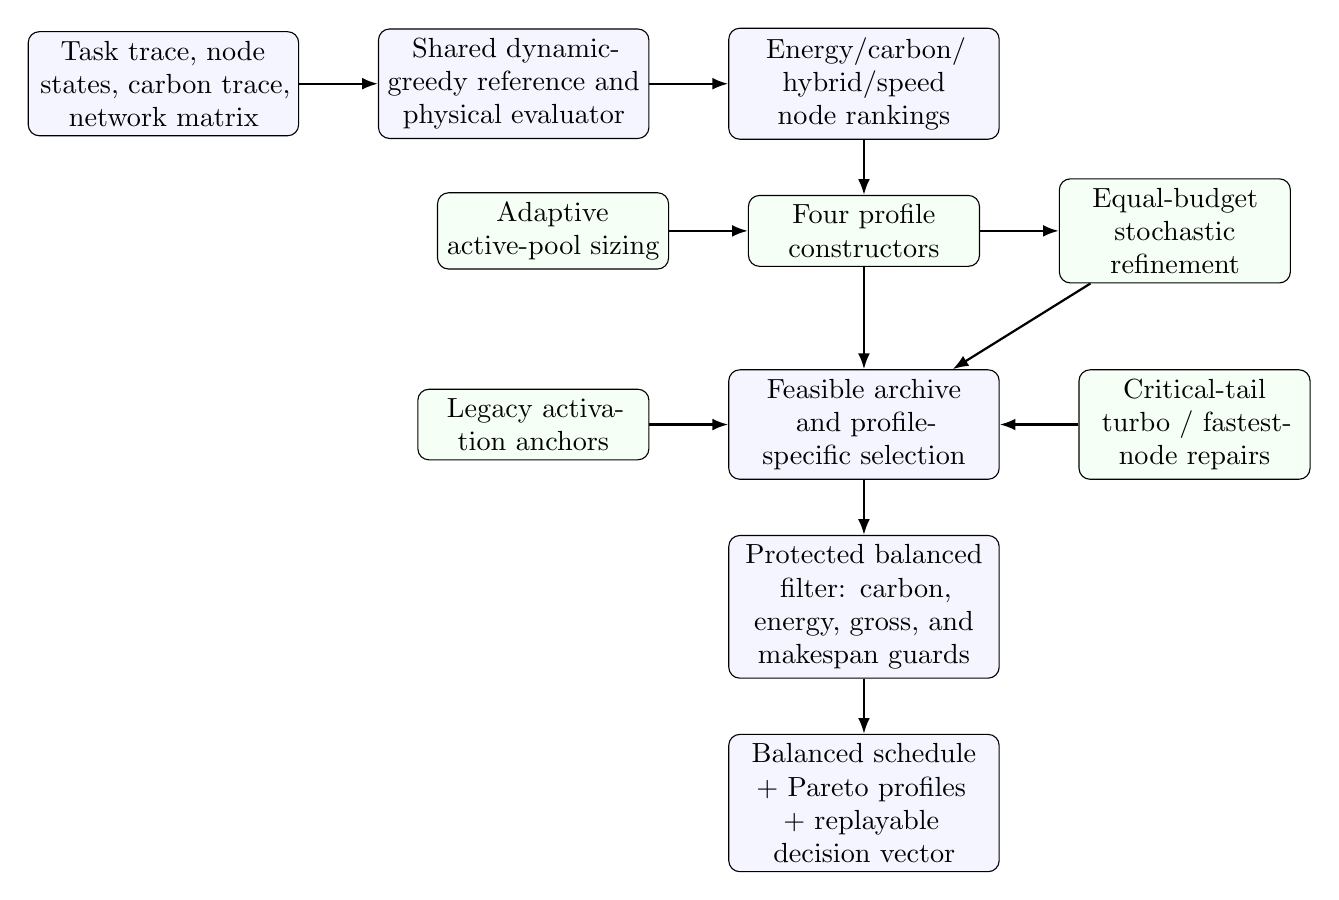
\begin{tikzpicture}[
node distance=7mm and 10mm,
box/.style={draw,rounded corners,align=center,minimum height=9mm,text width=3.2cm,fill=blue!4},
small/.style={draw,rounded corners,align=center,minimum height=8mm,text width=2.7cm,fill=green!4},
arrow/.style={-{Latex[length=2mm]},thick},
]
\node[box] (inputs) {Task trace, node states, carbon trace, network matrix};
\node[box,right=of inputs] (ref) {Shared dynamic-greedy reference and physical evaluator};
\node[box,right=of ref] (pool) {Energy/carbon/\\hybrid/speed\\node rankings};
\node[small,below=of pool] (profiles) {Four profile constructors};
\node[small,left=of profiles] (adaptive) {Adaptive active-pool sizing};
\node[small,right=of profiles] (search) {Equal-budget stochastic refinement};
\node[box,below=13mm of profiles] (archive) {Feasible archive and profile-specific selection};
\node[small,left=of archive] (legacy) {Legacy activation anchors};
\node[small,right=of archive] (tail) {Critical-tail turbo / fastest-node repairs};
\node[box,below=of archive] (guard) {Protected balanced filter: carbon, energy, gross, and makespan guards};
\node[box,below=of guard] (output) {Balanced schedule + Pareto profiles + replayable decision vector};
\draw[arrow] (inputs) -- (ref);
\draw[arrow] (ref) -- (pool);
\draw[arrow] (pool) -- (profiles);
\draw[arrow] (adaptive) -- (profiles);
\draw[arrow] (profiles) -- (search);
\draw[arrow] (profiles) -- (archive);
\draw[arrow] (search) -- (archive);
\draw[arrow] (legacy) -- (archive);
\draw[arrow] (tail) -- (archive);
\draw[arrow] (archive) -- (guard);
\draw[arrow] (guard) -- (output);
\end{tikzpicture}%
}
\caption{Execution flow of the frozen \method scheduler used in the reported experiments. All candidate schedules are evaluated by the same external simulator used for the baselines.}
\label{fig:workflow}
\end{figure*}

\subsection{Profile-aware construction}

For each task, a constructor considers a ranked subset of feasible nodes and a profile-specific set of DVFS/time-shift actions. Candidate nodes are ranked by static estimates of energy, carbon, speed, or a hybrid score. Within a selected pool, the constructor enumerates feasible actions and computes four local attributes: incremental energy, incremental carbon, normalized finish time, and whether a new node must be activated. Each attribute is min--max normalized over the current task's options.

Let $\kappa_i$ denote deadline criticality,
\begin{equation}
\kappa_i=\min\left(1,\frac{T^{\mathrm{fast}}_i}{\max(d_i-a_i,T^{\mathrm{fast}}_i,\epsilon)}\right),
\label{eq:criticality}
\end{equation}
where $T^{\mathrm{fast}}_i$ is the fastest runtime among the enumerated options. Each profile starts from a base weight vector $\mathbf{b}^{(p)}=(b_E,b_C,b_T,b_A)$. The finish-time weight increases with criticality,
\begin{equation}
\omega_T^{(p,i)}=\min\left(0.88,b_T^{(p)}+0.40\kappa_i\right),
\end{equation}
and the remaining weight is redistributed proportionally over energy, carbon, and activation:
\begin{equation}
(\omega_E,\omega_C,\omega_A)=
\frac{1-\omega_T}{b_E+b_C+b_A}(b_E,b_C,b_A).
\label{eq:profile-weights}
\end{equation}
The local option score is
\begin{equation}
S_{i,o}^{(p)}=\omega_E \hat{E}_{i,o}+\omega_C \hat{C}_{i,o}+\omega_T \hat{T}_{i,o}+\omega_A \hat{A}_{i,o},
\label{eq:local-score}
\end{equation}
and the lowest-scoring feasible option is reserved before the next task is processed. Tasks are considered by arrival time, then deadline, then descending work, which preserves the time structure of the trace while giving earlier deadlines precedence within an arrival batch.

\begin{table}[t]
\centering
\caption{Base profile weights and principal control choices. The finish weight is increased by Eq.~\eqref{eq:profile-weights} for critical tasks.}
\label{tab:profiles}
\scriptsize
\setlength{\tabcolsep}{3.5pt}
\begin{tabularx}{\linewidth}{lccccY}
\toprule
Profile & $b_E$ & $b_C$ & $b_T$ & $b_A$ & Main DVFS choices \\
\midrule
Balanced & 0.34 & 0.34 & 0.27 & 0.05 & eco, balanced, turbo \\
Carbon-guarded & 0.18 & 0.57 & 0.20 & 0.05 & eco, balanced, performance \\
Energy-guarded & 0.58 & 0.17 & 0.20 & 0.05 & eco-low, eco, balanced \\
Latency-guarded & 0.12 & 0.08 & 0.75 & 0.05 & performance, turbo \\
\bottomrule
\end{tabularx}
\end{table}

The allowed temporal-shift actions also depend on service class. Urgent tasks are never deliberately delayed. Standard tasks can use performance/balanced execution, while flexible tasks expose larger shift fractions in carbon- and balanced-oriented profiles. This keeps temporal carbon shifting tied to explicit slack instead of applying the same deferral rule to every task.

\subsection{Workload-adaptive active pools}

A fixed active-pool size behaves poorly across both sparse and contention-heavy workloads. \method estimates the required pool size from the maximum demand observed in a sliding 30-minute arrival window. Let $T_i^{\mathrm{turbo}}$ be the fastest feasible turbo runtime of task $i$, and let $\mathcal{W}(t)$ be the tasks arriving in $[t,t+1800)$. The pressure estimate is
\begin{equation}
D=\max_t\frac{\sum_{i\in\mathcal{W}(t)}T_i^{\mathrm{turbo}}}{1800}.
\end{equation}
The representative-regime pool size is
\begin{equation}
K=\mathrm{clip}\left(\left\lceil\frac{D}{0.75}\right\rceil,1,8\right),
\label{eq:pool-size}
\end{equation}
with at least two nodes for the latency profile. Energy-, carbon-, hybrid-, and speed-ranked pools use this value to generate four adaptive constructors. The search additionally evaluates balanced pools of sizes $1,2,3,4,6$ across the four ranking criteria and latency pools of sizes $1$--$4$ across energy, carbon, and hybrid rankings. These deterministic candidates are useful because they directly expose consolidation versus headroom choices before stochastic search begins.

\subsection{Equal-budget refinement and Pareto archive}

Let $B$ denote the externally assigned objective-call budget. The search begins with the dynamic-greedy anchor, uniform and efficiency-oriented pool vectors, four profile constructors, and criticality repairs. It then alternates between two low-cost perturbation modes until the allocated budget is consumed. Global diversification adds Gaussian noise to the anchor. Grouped mutation selects a contiguous task group and perturbs only node, DVFS, and temporal keys consistent with the active profile; leaders are refreshed periodically from the current archive. The grouped operator preserves useful constructor structure and avoids repeatedly randomizing all $3N$ coordinates.

Every evaluated vector is stored once using a rounded vector key. Feasible records are compared by the physical objective tuple in Eq.~\eqref{eq:objective-vector}; a record is non-dominated if no other feasible record is no worse in all six metrics and strictly better in at least one. The same archive is used for the four profile outputs, which avoids separate optimizer runs for carbon, energy, and latency.

Profile selection uses ratios to the dynamic-greedy reference. For the balanced profile, for example,
\begin{align}
U_{\mathrm{bal}} ={}& \max(R_C,R_E,R_T)+0.25(R_C+R_E)+0.25R_T \\
&+45\,[R_T-1.01]_+ + G + 5\times10^{-5}V_{\mathrm{mig}},
\label{eq:balanced-utility}
\end{align}
where $R_C=C_{\mathrm{ctrl}}/C_{\mathrm{ctrl}}^{\mathrm{ref}}$, $R_E=E_{\mathrm{ctrl}}/E_{\mathrm{ctrl}}^{\mathrm{ref}}$, $R_T=T_{\max}/T_{\max}^{\mathrm{ref}}$, and
\begin{equation}
G=30[R_{E,g}-1.01]_+ +30[R_{C,g}-1.01]_+
\end{equation}
penalizes gross-energy and gross-carbon regressions. Carbon-, energy-, and latency-guarded profiles use analogous utilities with profile-specific caps. These utilities guide selection; the Pareto indicators reported later are computed from the unscalarized physical metrics.

\subsection{Protected critical-tail repair}
\label{sec:tail-repair}

The final stage targets a failure mode that is easy to miss in energy-oriented schedules: a small number of late tasks can determine makespan even when the rest of the schedule is efficient. Two deterministic activation anchors are first constructed from the cloud node and the edge pool in region 3. The better feasible legacy anchor is retained as a reference. The balanced pre-repair schedule and the legacy anchor are each evaluated with a returned schedule and sorted by decreasing finish time.

For tail sizes $h\in\{1,2,4,8\}$, two repair vectors are generated from each base schedule. The first sets the $h$ latest-finishing tasks to turbo DVFS with no temporal shift. The second additionally moves each selected task to its fastest feasible turbo node. This produces 16 explicit tail candidates. Together with two legacy templates and two schedule-producing tail analyses, the stage reserves exactly 20 objective calls. Consequently, the earlier search receives $B-20$ calls and the complete method still consumes exactly $B$ calls.

The balanced output is chosen from feasible records satisfying all of the following fixed guards:
\begin{align}
C_{\mathrm{ctrl}} &\le C_{\mathrm{ctrl}}^{\mathrm{DG}}, \\
E_{\mathrm{ctrl}} &\le 1.10 E_{\mathrm{ctrl}}^{\mathrm{base}}, \\
C_{\mathrm{gross}} &\le C_{\mathrm{gross}}^{\mathrm{DG}}, \\
E_{\mathrm{gross}} &\le 1.05 E_{\mathrm{gross}}^{\mathrm{base}}, \\
T_{\max} &\le 1.01 T_{\max}^{\mathrm{DG}}, \\
(E_{\mathrm{gross}},C_{\mathrm{gross}},T_{\max})
&\le 1.05(E_{\mathrm{gross}},C_{\mathrm{gross}},T_{\max})^{\mathrm{legacy}}.
\label{eq:protected-guards}
\end{align}
Among candidates that pass Eq.~\eqref{eq:protected-guards}, selection is lexicographic in makespan, gross energy, gross carbon, and controllable energy. If no repair passes, the pre-repair balanced anchor is retained. The guard therefore cannot force a worse repair merely because a tail candidate is faster.

\begin{algorithm}[t]
\caption{Guarded multi-profile search in \method}
\label{alg:hcsmo}
\begin{algorithmic}[1]
\Require Shared simulator $\mathcal{S}$, task set $\mathcal{T}$, evaluation budget $B$, search seed $s$
\Ensure Balanced schedule, four profile schedules, non-dominated archive
\State Evaluate the shared dynamic-greedy anchor and initialize archive $\mathcal{A}$
\State Build energy, carbon, hybrid, speed, and workload-adaptive pool candidates
\State Evaluate deterministic profile and joint constructors
\State Allocate $B-20$ calls to base search and grouped stochastic refinement
\While{base budget remains}
    \State Cycle through the four profiles
    \State Generate anchor diversification or profile-consistent grouped mutation
    \State Evaluate with $\mathcal{S}$ and update $\mathcal{A}$ and profile leaders
\EndWhile
\State Evaluate region-3 cloud and edge legacy activation anchors
\For{base $\in\{$balanced anchor, legacy anchor$\}$}
    \State Sort tasks by decreasing finish time
    \For{$h\in\{1,2,4,8\}$}
        \State Evaluate turbo/no-shift repair on the $h$ latest tasks
        \State Evaluate fastest-feasible-node + turbo/no-shift repair
    \EndFor
\EndFor
\State Form the non-dominated set from feasible records
\State Apply Eq.~\eqref{eq:protected-guards} to balanced candidates
\State Return the fastest protected candidate and the four profile outputs
\end{algorithmic}
\end{algorithm}
% ---- END sections/04_method.tex ----
% ---- BEGIN sections/05_algorithmic_properties.tex ----
\section{Algorithmic Properties and Computational Cost}
\label{sec:properties}

The deployed scheduler combines deterministic construction, stochastic search, and an external feasibility-aware simulator. This structure supports several implementation guarantees, but it does not imply global convergence for the mixed discrete/continuous scheduling problem. We therefore state only properties that follow directly from the frozen implementation.

\subsection{Feasibility and deadline handling}

Resource feasibility is enforced during reservation construction. For every decoded task, the evaluator searches for the earliest start time at which the requested CPU and memory fit the existing reservations on the selected node. If the resulting completion exceeds the deadline, the common repair first removes temporal shifting and raises the selected node to the performance state; if necessary, all feasible nodes are checked under the same repair and the earliest completion is selected. Final profile selection excludes any record with a positive deadline-miss ratio or non-zero total tardiness. Thus, the schedules reported for \method are feasible by construction under the same repair logic available to every comparator. This is an evaluator property, not a claim that arbitrary instances are always feasible.

\subsection{Exact objective-call accounting}

Let $B$ be the budget assigned to a method in a scenario. \method reserves 20 objective calls for two legacy anchors, two schedule-producing tail analyses, and 16 critical-tail candidates, while its earlier search receives $B-20$ calls. No post-search replay call is counted as a search objective call. The final suite verifies the counter directly for every equal-budget run. As a result, comparisons with ECO-PSO, TM-MOAOA, the adapted metaheuristics, NSGA-II, and PPO use the same number of calls to the external objective evaluator for a given scenario.

\subsection{Search cost}

Let $C_{\mathrm{eval}}(N,M)$ denote the cost of evaluating one $3N$-dimensional decision vector on $M$ heterogeneous nodes. The dominant work is reservation placement, migration calculation, and piecewise power/carbon integration. \method performs exactly $B$ such evaluations, so its dominant cost is
\begin{equation}
\mathcal{O}\left(B\,C_{\mathrm{eval}}(N,M)\right).
\end{equation}
Candidate construction adds node ranking and local option enumeration. With a bounded active-pool size $K\le 8$, the constructor overhead is approximately $\mathcal{O}(NK|\mathcal{F}|)$ after node rankings are available. The critical-tail stage evaluates a constant number of candidates because the tail-size set is fixed to $\{1,2,4,8\}$. Archive storage grows linearly with the number of unique evaluated vectors; storing all decision vectors therefore requires $\mathcal{O}(BN)$ values in the reference implementation.

The wall-clock results in Section~\ref{sec:runtime-results} are more informative than asymptotic notation for practical use, because the compared methods differ in Python-level search bookkeeping and PPO additionally incurs neural-network inference and updates. We therefore report both objective-call equality and measured decision time.

\subsection{Protected-selection property}

The final repair stage cannot replace the pre-repair balanced anchor with a candidate that violates the fixed guard set in Eq.~\eqref{eq:protected-guards}. When the admissible set is empty, the base anchor is returned. When it is non-empty, the selected candidate is the fastest member of that set. This yields a simple conditional property: \emph{tail repair can change the deployed balanced schedule only inside the declared carbon, energy, gross-accounting, and makespan protection envelope}. The property is intentionally local to the evaluated candidate set and should not be interpreted as a global optimality theorem.
% ---- END sections/05_algorithmic_properties.tex ----
% ---- BEGIN sections/06_experimental_methodology.tex ----
\section{Experimental Methodology}
\label{sec:experimental}

\subsection{Trace-derived workloads and evaluation tracks}

The workload scenarios are derived from two public production traces: the Google cluster workload released in 2011 and Alibaba Cluster Trace v2017 \cite{reiss2012google,cheng2018alibaba,shahmirzadi2024analyzing}. We use two scenario families for each dataset. \emph{Trace-dynamic} scenarios retain the trace-derived resource and timing structure, whereas \emph{flexible-dynamic} scenarios expose additional scheduling slack while preserving the task resource characteristics. Source task identifiers remain unique in every scenario and are carried into the saved schedule, allowing row-level replay.

The evaluation uses two separate tracks because sparse representative workloads and SLA stress answer different questions. The representative track contains 12 frozen scenarios: two datasets $\times$ two families $\times$ task counts of 30, 60, and 90, all on 30 nodes. Scenario seeds 811, 823, and 827 are tied to the three task counts. These files are byte-for-byte frozen inputs to the final benchmark.

The SLA-constrained track contains 12 controlled stress cells on 50 nodes and 150 tasks. Four base scenarios (two datasets $\times$ two families) are evaluated with workload seeds 6000, 6101, and 6102. Seed 6000 is the original SLA-constrained scenario. Seeds 6101 and 6102 apply service-class-stratified permutations to task arrival times; CPU work, CPU/memory requests, migration state, service class, source ID, and SLA slack are unchanged, and each deadline is reconstructed as the new arrival plus the unchanged slack. We therefore treat these cells as \emph{controlled SLA-constrained workload-seed replications}, not as independent untouched trace replays.

\begin{table*}[t]
\centering
\caption{Final experimental design. Search seeds are nested algorithmic repetitions; paired inference is performed after aggregating within scenario/workload cells.}
\label{tab:design}
\scriptsize
\setlength{\tabcolsep}{3pt}
\begin{tabularx}{\textwidth}{p{2.15cm}Y p{1.45cm}C{0.85cm}C{0.85cm}p{2.55cm}C{1.25cm}}
\toprule
Track & Datasets & Families & Nodes & Tasks & Workload/scenario seeds & Calls \\
\midrule
Representative & Google2011v2; Alibaba2017 & trace; flexible & 30 & 30 & 811 & 156 \\
 &  &  & 30 & 60 & 823 & 216 \\
 &  &  & 30 & 90 & 827 & 276 \\
SLA stress & Google2011v2; Alibaba2017 & trace; flexible & 50 & 150 & 6000, 6101, 6102 & 396 \\
\bottomrule
\end{tabularx}
\end{table*}

\subsection{Carbon, network, and power environment}

The environment contains six regions. Carbon intensity comes from a half-hourly six-region NESO forecast trace spanning 1--8 January 2024; the 336 slots per region are replayed cyclically over one week by the simulator. Inter-region placement is charged through the frozen network matrix using round-trip latency, bandwidth, and transfer energy. Same-region execution incurs no migration transfer. Inter-region RTTs range from 8 to 38~ms, bandwidth from 5 to 25~Gbit/s, and transfer energy is 0.06~Wh/GiB. The matrix also stores jitter bounds for provenance, but the deterministic evaluator uses the declared base RTT and bandwidth values so that identical decision vectors replay exactly.

Table~\ref{tab:power-model} summarizes the base node classes. Regional PUE ranges from 1.12 to 1.22 across the six regions. The simulator accounts for active dynamic power, standby/sleep states, minimum up/sleep durations, predictive wake latency, and wake energy. The same control model is exposed to every method.

\begin{table*}[t]
\centering
\caption{Representative node-class power parameters used by the shared simulator. CPU/memory capacities are normalized trace-scale capacities.}
\label{tab:power-model}
\scriptsize
\setlength{\tabcolsep}{4pt}
\begin{tabular}{lcccccccc}
\toprule
Type & CPU & Mem. & Idle & Dyn. & Stby. & Sleep & Wake & Wake E. \\
 & & & (W) & (W) & (W) & (W) & (s) & (Wh) \\
\midrule
Edge & 0.25 & 0.25 & 40 & 60 & 8 & 3.2 & 5 & 0.174 \\
Regional & 0.50 & 0.50 & 90 & 130 & 18 & 7.2 & 15 & 1.146 \\
Cloud & 1.00 & 1.00 & 180 & 240 & 36 & 14.4 & 30 & 4.375 \\
\bottomrule
\end{tabular}
\end{table*}

The five-state DVFS multipliers are shown in Table~\ref{tab:dvfs}. They are applied uniformly across methods. The performance state is the nominal baseline; turbo raises speed by 10\% with higher idle/dynamic power, while eco and eco-low trade runtime for lower power.

\begin{table}[t]
\centering
\caption{Five-state DVFS control shared by all schedulers.}
\label{tab:dvfs}
\small
\begin{tabular}{lccc}
\toprule
State & Speed $\sigma_f$ & Idle mult. & Dynamic mult. \\
\midrule
Eco-low & 0.70 & 0.82 & 0.46 \\
Eco & 0.80 & 0.86 & 0.55 \\
Balanced & 0.90 & 0.92 & 0.70 \\
Performance & 1.00 & 1.00 & 1.00 \\
Turbo & 1.10 & 1.05 & 1.30 \\
\bottomrule
\end{tabular}
\end{table}

\subsection{Compared methods and fairness controls}

The main benchmark contains eight equal-budget methods. ECC-CEE, MEO, and Jellyfish-RTS are adapted implementations: their characteristic search logic is retained, but candidate schedules are represented and evaluated in the shared joint placement--time--DVFS space rather than by private method-specific simulators. This distinction is explicit because the comparison targets scheduling behavior under a common physical evaluator, not line-by-line reproduction of third-party source code.

\begin{table*}[t]
\centering
\caption{Methods in the main equal-budget benchmark.}
\label{tab:baselines}
\scriptsize
\setlength{\tabcolsep}{4pt}
\begin{tabularx}{\textwidth}{p{2.7cm}p{2.8cm}Y}
\toprule
Method & Family & Role in the comparison \\
\midrule
\method & Guarded multi-profile search & Proposed joint placement/time/DVFS scheduler with adaptive pools and critical-tail protection. \\
ECC-CEE-adapted \cite{zhai2024edge} & Carbon-aware edge--cloud & Adapted carbon/latency-oriented search under the common evaluator. \\
ECO-PSO-Joint \cite{pournazari2025multi} & PSO/metaheuristic & Joint-control PSO-style search with equal objective-call budget. \\
TM-MOAOA-Joint \cite{khaledian2025tm} & MCDM + metaheuristic & Joint-control adaptation of TOPSIS/MOAOA scheduling. \\
MEO-adapted \cite{pournazari2025carbon} & Multi-objective metaheuristic & Adapted carbon-aware multi-objective search. \\
Jellyfish-RTS-adapted \cite{nigade2024inference} & Latency-oriented metaheuristic & Adapted latency-sensitive evolutionary search. \\
NSGA-II \cite{deb2002nsga2} & Pareto evolutionary & Four-objective non-dominated sorting with crowding under the common decision vector. \\
PPO-Joint \cite{schulman2017ppo} & Deep RL & PPO policy over joint actions, imitation-warm-started without simulator calls, then trained/evaluated inside the same call budget. \\
\bottomrule
\end{tabularx}
\end{table*}

Three search seeds (42, 211, and 307) are used for every stochastic main method. These seeds are algorithmic repetitions, not independent workload samples. For paired statistical inference, metrics are first summarized within each scenario/workload cell; the 12 cells in each track are then the paired units. Every main method receives the same scenario file, node/power model, network and carbon traces, decoder, deadline repair, objective definitions, and objective-call budget shown in Table~\ref{tab:design}.

For diagnostic context, we additionally retain Dynamic Greedy, the historical H-CSMO-v3C implementation, and a constructor-only scheduler. Appendix controls include \emph{true uniform feasible random} and \emph{baseline-perturbed random (35\% mutation)}. The latter is deliberately not described as true random assignment because it mutates a baseline schedule rather than sampling uniformly from the feasible space.

\subsection{Metrics and statistical analysis}

The primary metrics are scheduler-controllable emissions $C_{\mathrm{ctrl}}$, scheduler-controllable energy $E_{\mathrm{ctrl}}$, gross fixed-horizon emissions $C_{\mathrm{gross}}$, gross fixed-horizon energy $E_{\mathrm{gross}}$, and makespan $T_{\max}$. We also report deadline-miss ratio, total tardiness, migration volume/energy/emissions, active-node count, wall-clock decision time, Pareto coverage, additive epsilon indicator, and normalized three-objective hypervolume. Hypervolume uses controllable carbon, controllable energy, and makespan after common normalization within each scenario.

The omnibus comparison uses the Friedman test across the eight methods. Pairwise comparisons between \method and each competitor use a two-sided Wilcoxon signed-rank test on paired scenario values, followed by Holm correction within each metric/track family. Effect size is the matched-pairs rank-biserial correlation computed from positive and negative signed ranks. A 5000-resample scenario bootstrap provides a confidence interval for the median paired difference. These analyses use scenario/workload cells as the statistical unit rather than treating the three search seeds as independent evidence.

\subsection{Ablation, sensitivity, and reproducibility}

The ablation study includes the full scheduler and equal-budget variants with critical-tail repair removed, adaptive active-pool logic removed, five-state DVFS removed, carbon shifting disabled, migration disabled, race-to-idle disabled, and the legacy protection guard removed. Constructor-only and historical-v3C results are reported as diagnostic references rather than equal-budget ablations. Sensitivity experiments cover evaluation budget, active-pool size, critical-tail size, makespan/energy protection guards, migration-energy threshold, carbon-shift cap, and DVFS policy. Parameters that are not active in the frozen implementation are not presented as tunable factors.

The complete experiment contains 576 main equal-budget runs and 1128 total run/reference/control items. Every completed run is atomically committed with a summary, decision vectors, schedules, evaluation log, per-file SHA-256 manifest, and completion sentinel. The final artifact audit verified all 1128 items. Independent replay of all 576 balanced main profiles reproduced the saved metrics exactly and the numeric schedules to a maximum absolute difference of $5.82\times10^{-11}$. The software environment used Python 3.12.13 on 64-bit Linux with NumPy 2.0.2, pandas 2.2.2, SciPy 1.16.3, Matplotlib 3.10.0, and CPU-only PyTorch 2.11.0.
% ---- END sections/06_experimental_methodology.tex ----
% ---- BEGIN sections/07_results.tex ----
\section{Results}
\label{sec:results}

The results are reported separately for the representative and SLA-constrained tracks. Within each scenario, lower carbon, energy, and makespan are better; method ranks are computed scenario by scenario before averaging. This avoids allowing a single high-magnitude scenario to dominate the comparison.

\subsection{Overall ranking on representative workloads}

Figure~\ref{fig:overall-ranks}a shows the average rank across the five primary metrics on the 12 representative scenarios. \method obtains an overall average rank of \good{1.98}, followed by ECC-CEE-adapted (3.38), NSGA-II (3.65), Jellyfish-RTS-adapted (3.84), MEO-adapted (3.85), TM-MOAOA-Joint (5.31), PPO-Joint (6.40), and ECO-PSO-Joint (7.58). The result is not driven by a single objective: \method has the best average rank for controllable carbon (1.67), controllable energy (1.92), gross carbon (1.67), gross energy (1.92), and makespan (2.75). It places first in 10/12 representative cells for both controllable and gross carbon, 8/12 for both energy measures, and 5/12 for makespan.

\begin{figure*}[t]
\centering
\begin{subfigure}[t]{0.49\textwidth}
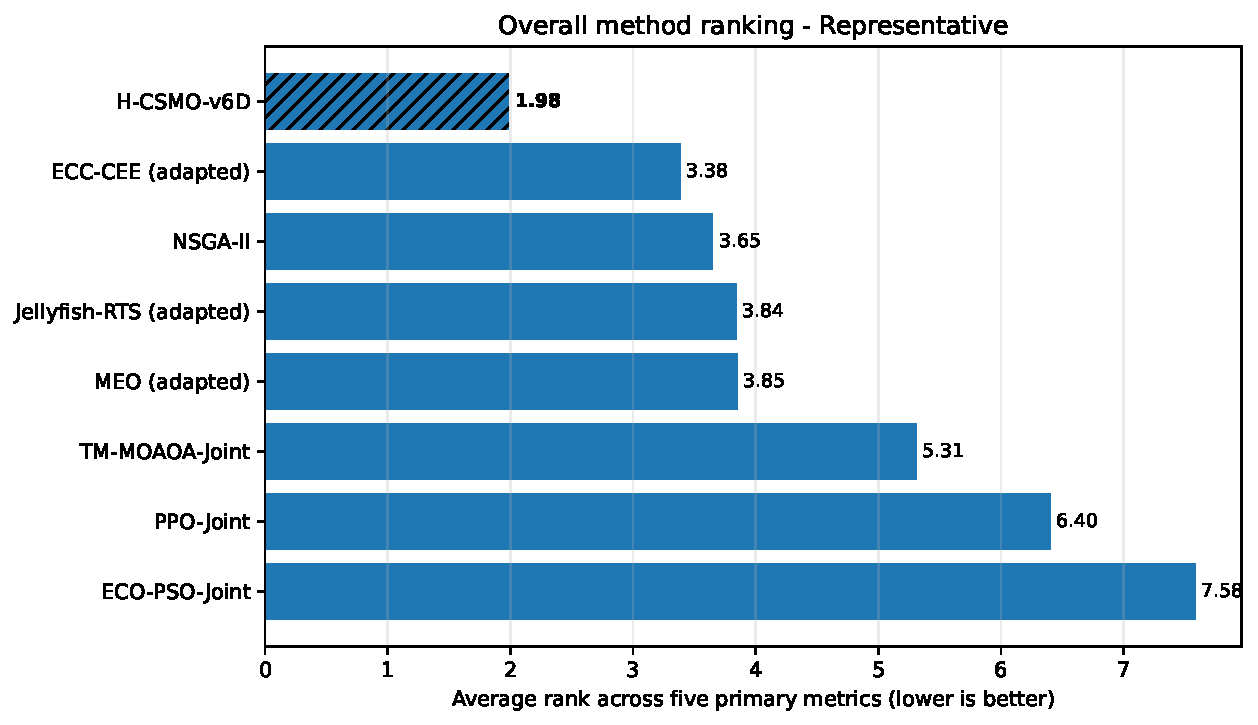
\includegraphics[width=\linewidth]{fig01_overall_average_rank_representative.pdf}
\caption{Representative track.}
\end{subfigure}\hfill
\begin{subfigure}[t]{0.49\textwidth}
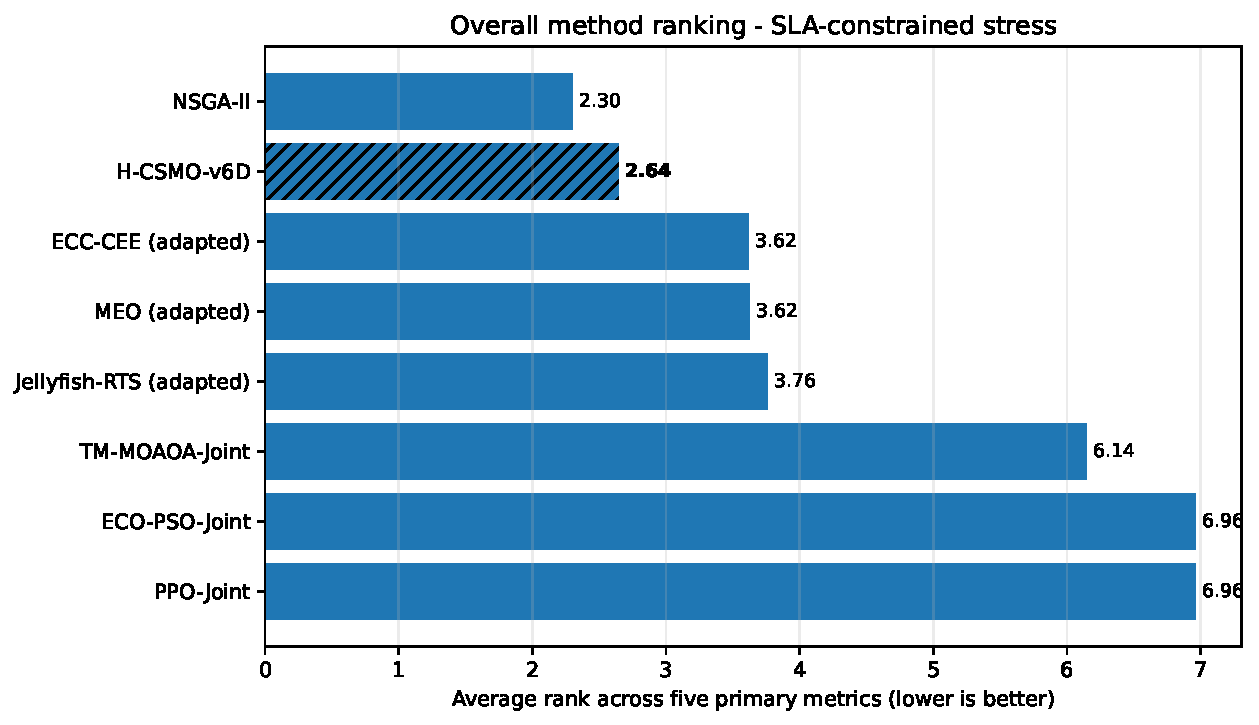
\includegraphics[width=\linewidth]{fig01_overall_average_rank_sla_stress.pdf}
\caption{SLA-constrained stress track.}
\end{subfigure}
\caption{Average rank across the five primary metrics. Lower rank is better. \method leads the representative track and ranks second under SLA stress.}
\label{fig:overall-ranks}
\end{figure*}

Table~\ref{tab:overall-ranks} makes the distinction between the two tracks explicit. On representative workloads, \method is the strongest method by the aggregate rank used here. Under SLA stress, NSGA-II moves to first overall, while \method remains second and retains the best average makespan rank.

\begin{table*}[t]
\centering
\caption{Overall average rank across the five primary metrics (lower is better). Bold indicates the best rank in each track.}
\label{tab:overall-ranks}
\small
\begin{tabular}{lcc}
\toprule
Method & Representative & SLA stress \\
\midrule
\method & \good{1.98} & 2.64 \\
ECC-CEE-adapted & 3.38 & 3.62 \\
ECO-PSO-Joint & 7.58 & 6.96 \\
TM-MOAOA-Joint & 5.31 & 6.14 \\
MEO-adapted & 3.85 & 3.63 \\
Jellyfish-RTS-adapted & 3.84 & 3.76 \\
NSGA-II & 3.65 & \good{2.30} \\
PPO-Joint & 6.40 & 6.96 \\
\bottomrule
\end{tabular}
\end{table*}

The representative heatmap in Fig.~\ref{fig:heatmaps}a explains where the rank advantage comes from. Relative to the strongest competing method in each cell, the median \method improvement is \good{21.99\%} for controllable carbon and 1.95\% for controllable energy. Once the fixed infrastructure floor is included, the corresponding median advantages narrow to 0.39\% for gross carbon and 0.23\% for gross energy, which is expected from Eqs.~\eqref{eq:controllable-energy}--\eqref{eq:carbon-layers}. Median makespan is essentially tied with the strongest per-cell competitor.

The principal exceptions are confined to the four sparse 30-task cells. In the two Alibaba cells, a specialist competitor becomes the carbon leader; in the two Google cells, an energy-specialized schedule becomes the energy leader. Figure~\ref{fig:heatmaps}a reports the exact cell-level magnitudes rather than averaging them away. At 60 and 90 tasks, all eight representative cells remain within 1\% of the strongest comparator on every primary metric, while preserving the aggregate rank advantage of \method. This scale separation is examined further in Section~\ref{sec:discussion}.

\begin{figure*}[t]
\centering
\begin{subfigure}[t]{0.49\textwidth}
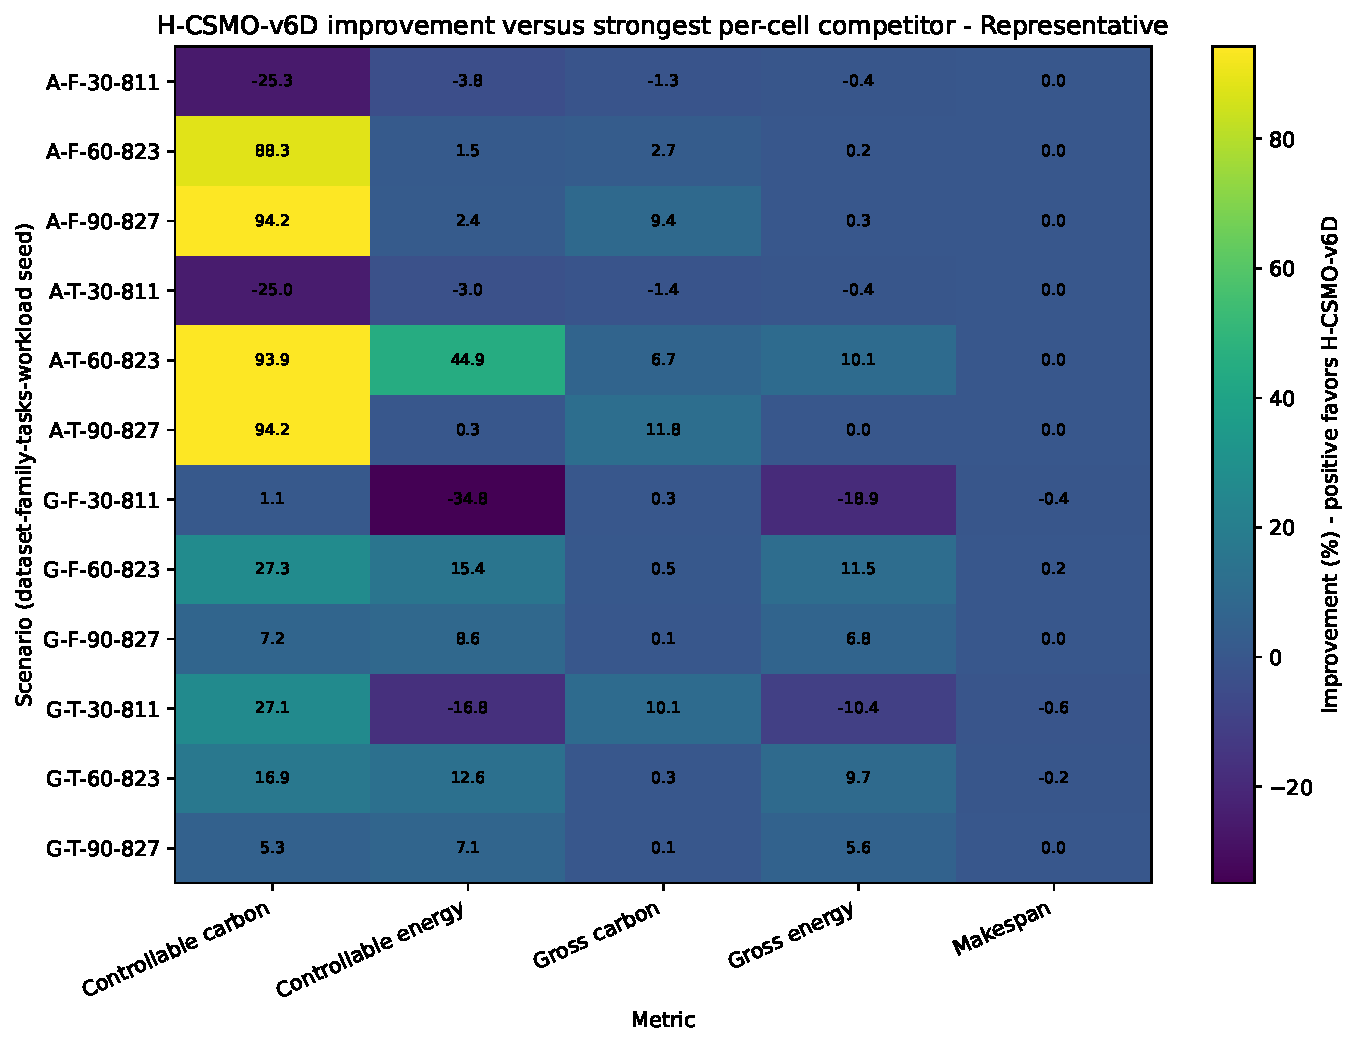
\includegraphics[width=\linewidth]{fig03_cell_improvement_heatmap_representative.pdf}
\caption{Representative scenarios.}
\end{subfigure}\hfill
\begin{subfigure}[t]{0.49\textwidth}
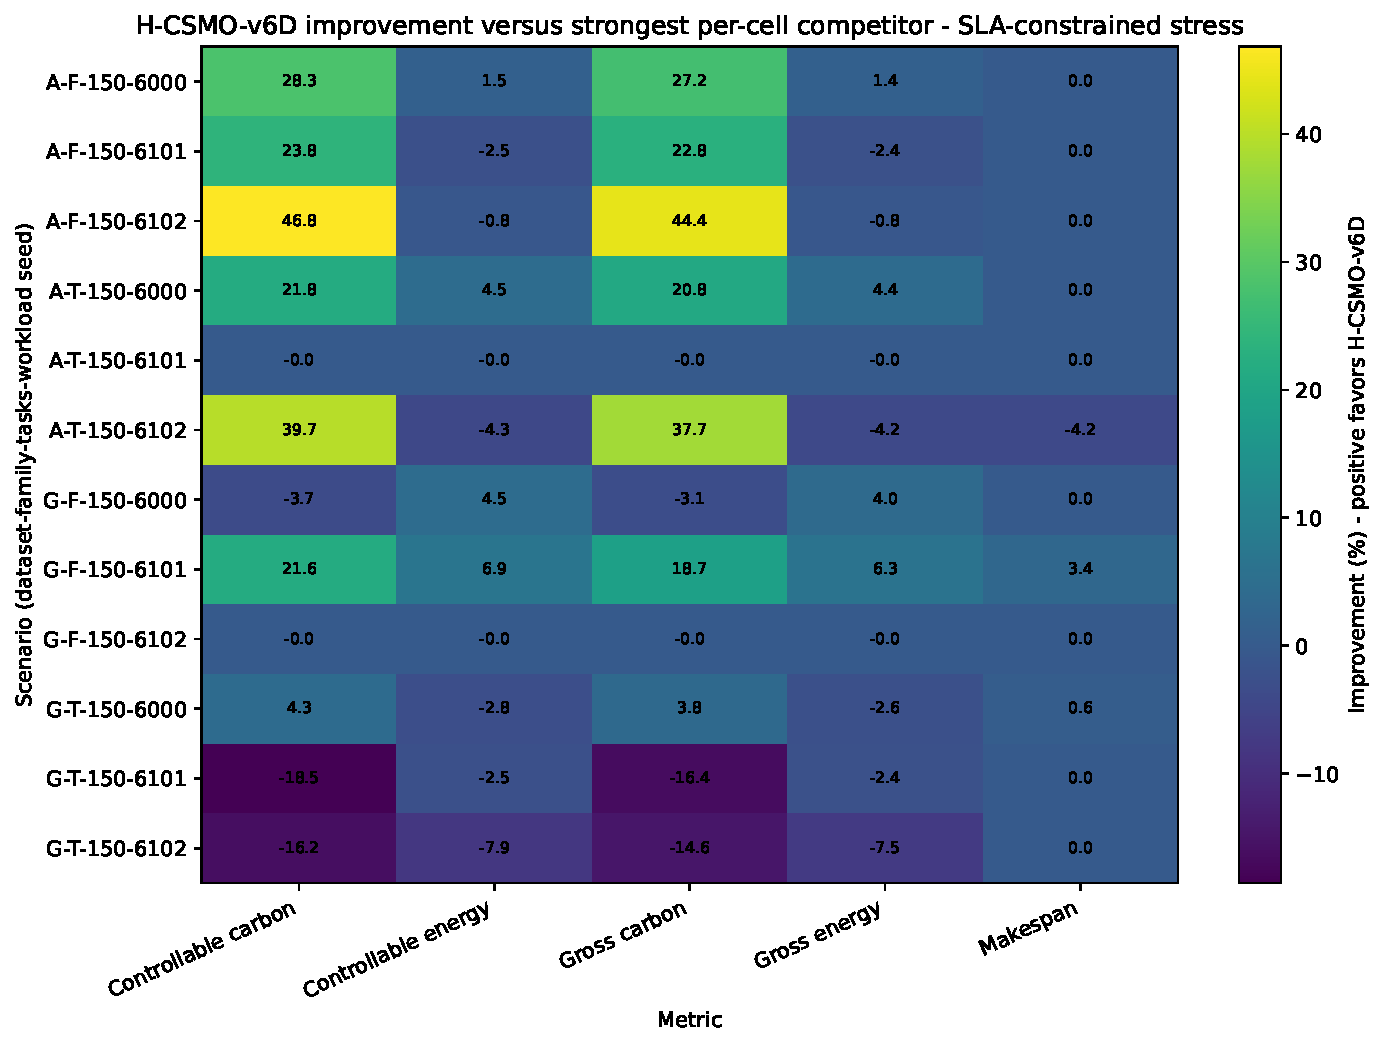
\includegraphics[width=\linewidth]{fig03_cell_improvement_heatmap_sla_stress.pdf}
\caption{SLA stress scenarios.}
\end{subfigure}
\caption{Per-cell improvement of \method relative to the strongest competitor for each metric. Positive values favor \method. The full matrix is shown to preserve workload-level variation.}
\label{fig:heatmaps}
\end{figure*}

\subsection{SLA-constrained stress performance}

The SLA track changes the relative order of the strongest methods. NSGA-II obtains the best overall rank (2.30), followed by \method (2.64). The proposed scheduler nevertheless remains highly competitive across the five metrics: its average ranks are 2.42 for controllable carbon, 3.00 for controllable energy, 2.42 for gross carbon, 3.00 for gross energy, and \good{2.38} for makespan. The last value is the best average makespan rank among all eight methods.

Against the strongest competitor selected independently in each SLA cell, \method has a median controllable-carbon improvement of \good{12.95\%} and a median gross-carbon improvement of \good{11.24\%}. Energy is effectively at parity at the track median: controllable energy is 0.40\% higher and gross energy 0.38\% higher than the strongest per-cell value. Median makespan difference is zero. This pattern clarifies the role of the profile search under contention: \method preserves a strong carbon/makespan operating point, while NSGA-II more often finds the lowest-energy point in the same scenario.

The workload-level view remains important. Six of the 12 SLA cells fall within 1\% of the strongest comparator on all five primary metrics. In the remaining cells, the competing leader is specialized on one or more individual axes; Fig.~\ref{fig:heatmaps}b retains the exact deviations. The next subsection shows that these single-profile exceptions do not translate into a weaker trade-off set: the \method archive retains the highest normalized three-objective hypervolume throughout the SLA track.

\subsection{Pareto quality and hypervolume}
\label{sec:pareto-results}

The clearest cross-track result is obtained from the Pareto set rather than the single balanced profile. Figure~\ref{fig:hypervolume} shows the exact normalized three-objective hypervolume ranks using controllable carbon, controllable energy, and makespan. \method ranks \good{first in all 24 scenarios}: 12/12 representative cells and 12/12 SLA cells. This remains true in the SLA track even though NSGA-II has the better overall average single-profile rank.

\begin{figure*}[t]
\centering
\begin{subfigure}[t]{0.49\textwidth}
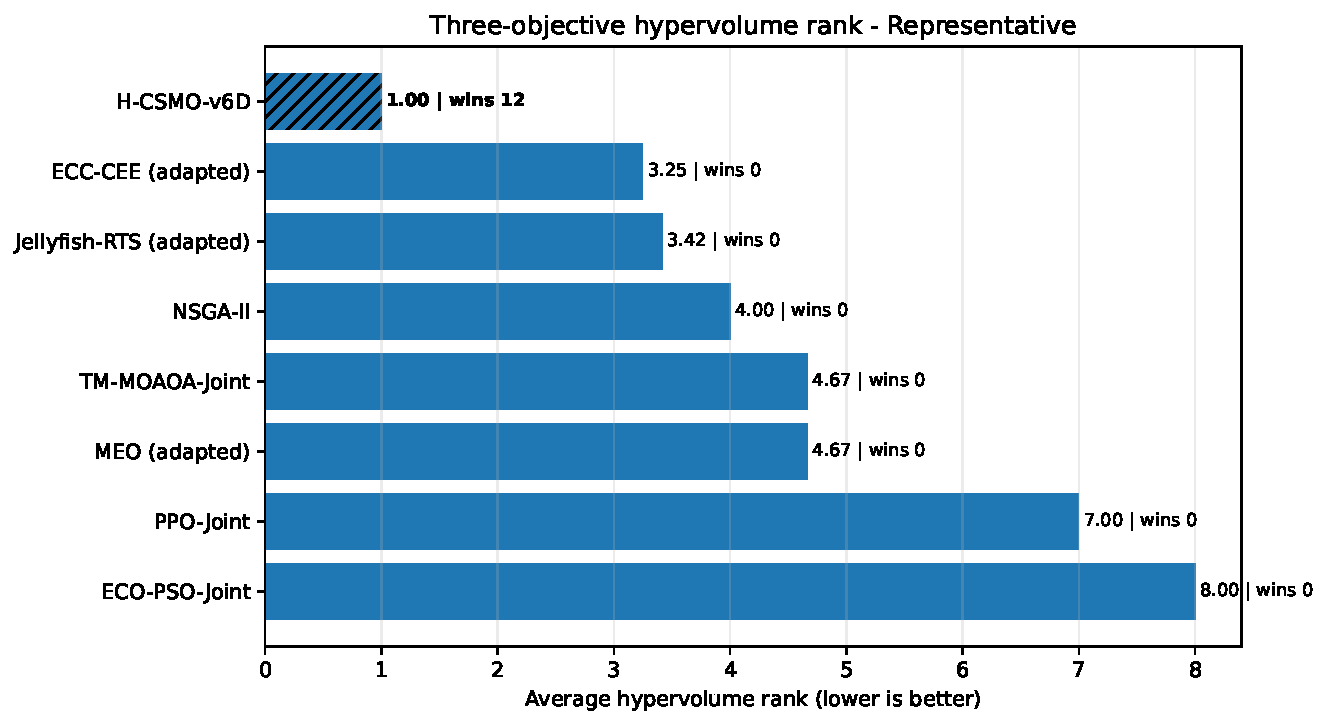
\includegraphics[width=\linewidth]{fig09_hypervolume_rank_representative.pdf}
\caption{Representative track.}
\end{subfigure}\hfill
\begin{subfigure}[t]{0.49\textwidth}
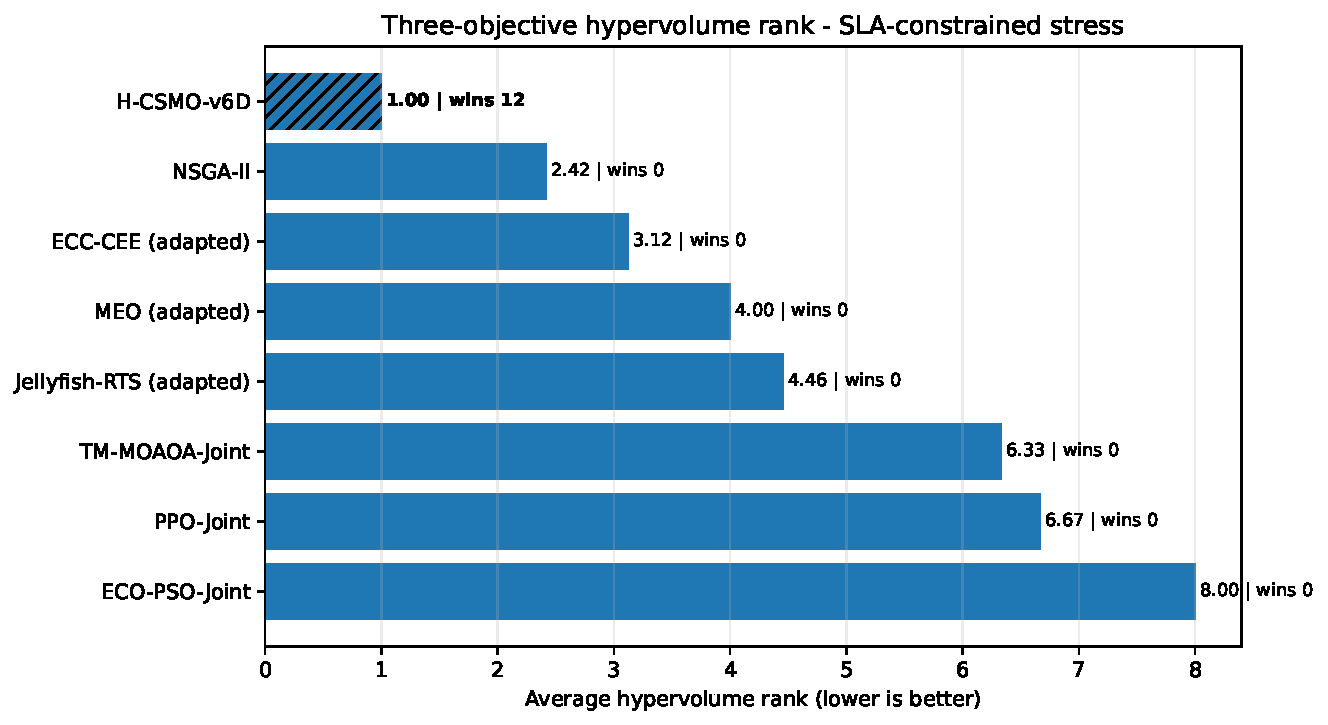
\includegraphics[width=\linewidth]{fig09_hypervolume_rank_sla_stress.pdf}
\caption{SLA stress track.}
\end{subfigure}
\caption{Rank of exact normalized three-objective hypervolume. \method attains rank 1 in every evaluated scenario.}
\label{fig:hypervolume}
\end{figure*}

Pareto coverage supports the same interpretation with more nuance. On representative workloads, the fraction of competitor front points dominated by the \method front has mean 0.869 and median 1.0. Under SLA stress, mean coverage decreases to 0.535 and median coverage to 0.420 because the strong NSGA-II/ECC-CEE/MEO/Jellyfish fronts retain non-dominated specialist points. The hypervolume remains higher because \method covers a broader balanced region of the normalized carbon--energy--makespan space. Example projections are shown in Fig.~\ref{fig:pareto-projection}.

\begin{figure*}[t]
\centering
\begin{subfigure}[t]{0.49\textwidth}
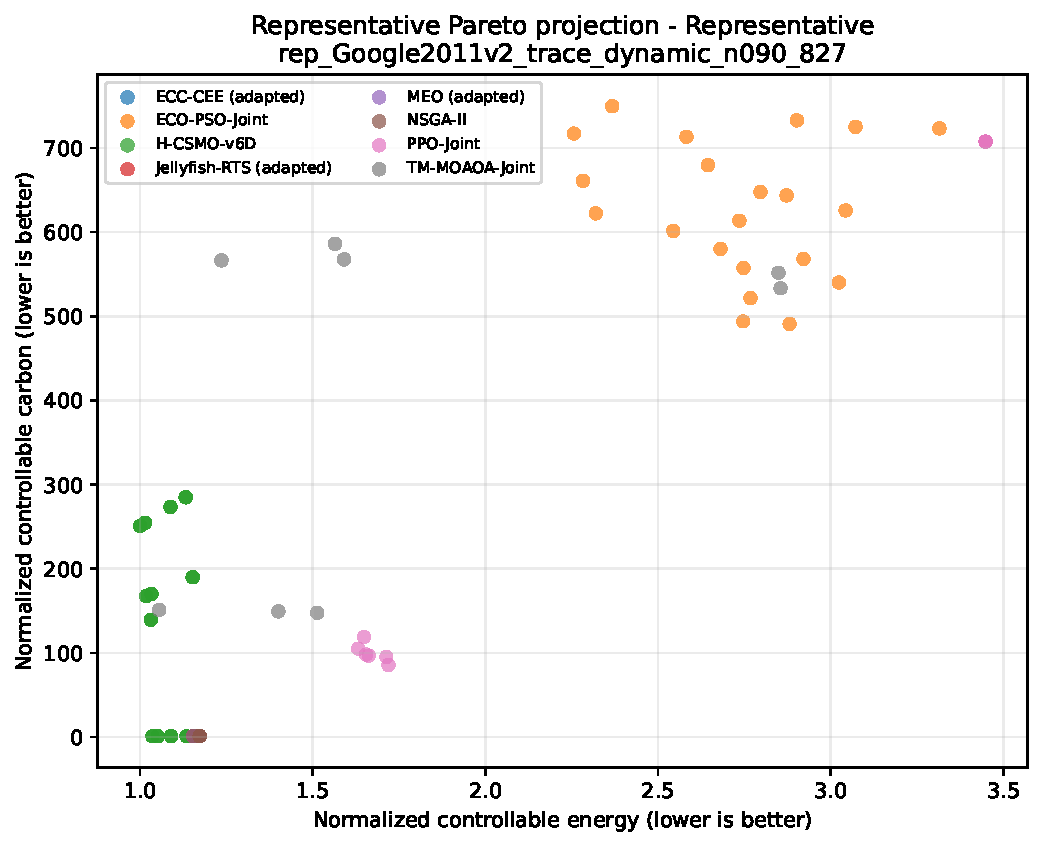
\includegraphics[width=\linewidth]{fig14_pareto_projection_representative.pdf}
\caption{Representative projection.}
\end{subfigure}\hfill
\begin{subfigure}[t]{0.49\textwidth}
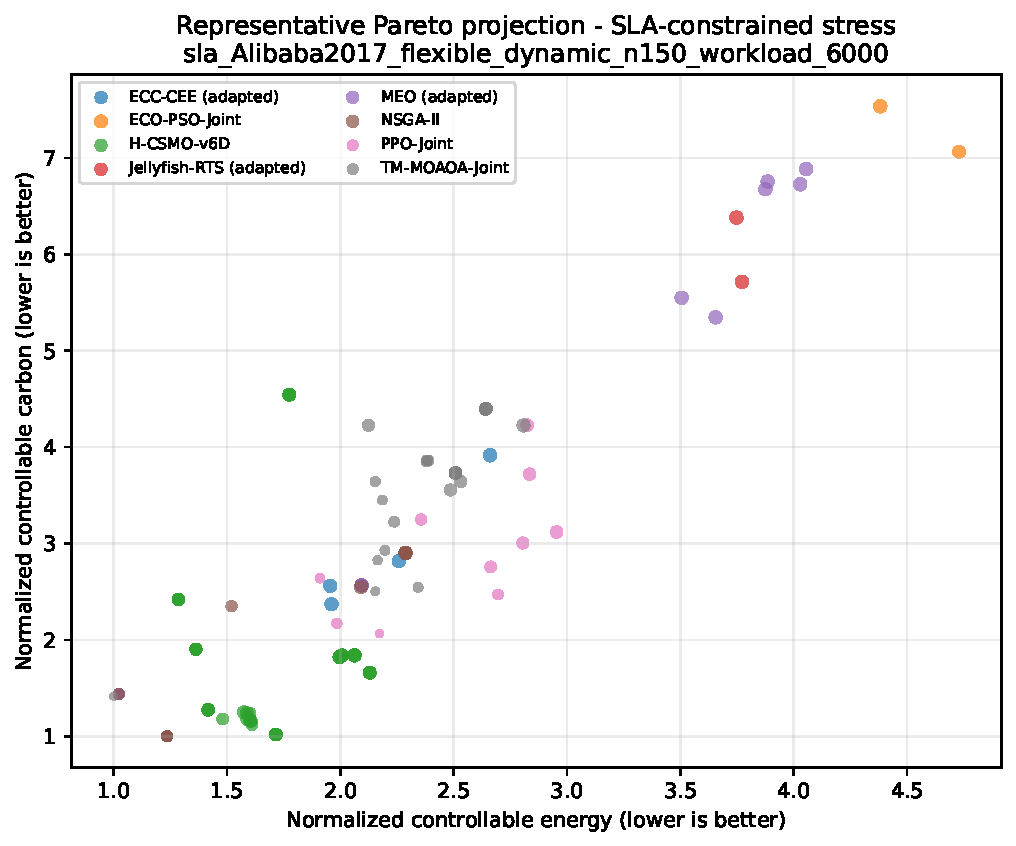
\includegraphics[width=\linewidth]{fig14_pareto_projection_sla_stress.pdf}
\caption{SLA-stress projection.}
\end{subfigure}
\caption{Two-dimensional projection of the three-objective Pareto sets. Marker size encodes the normalized makespan component used in the three-dimensional hypervolume.}
\label{fig:pareto-projection}
\end{figure*}

\subsection{Statistical evidence}
\label{sec:statistics-results}

The Friedman test rejects equal performance among the eight methods for every primary metric in both tracks ($p\le1.12\times10^{-7}$ on representative scenarios and $p\le8.35\times10^{-10}$ on SLA scenarios). Pairwise Wilcoxon--Holm results are summarized in Fig.~\ref{fig:significance}. On representative workloads, \method has a Holm-significant positive advantage in controllable and gross energy over six of seven competitors. Carbon advantages are Holm-significant over ECO-PSO, TM-MOAOA, and PPO; makespan is significantly better than TM-MOAOA. Against ECC-CEE and several strong Pareto/metaheuristic methods, the direction is often favorable but the 12 paired scenarios do not support a corrected $p<0.05$ claim for every metric.

Under SLA stress, the result is especially clean against three methods: ECO-PSO, TM-MOAOA, and PPO. \method is Holm-significantly better than each of them for all five primary metrics. The matched-pairs rank-biserial effects are 0.92--1.00 for these comparisons, indicating that the paired direction is consistent across most or all stress cells. Comparisons with NSGA-II, ECC-CEE, MEO, and Jellyfish-RTS are not uniformly significant, which is consistent with their stronger positions in the SLA ranking.

\begin{figure*}[t]
\centering
\begin{subfigure}[t]{0.49\textwidth}
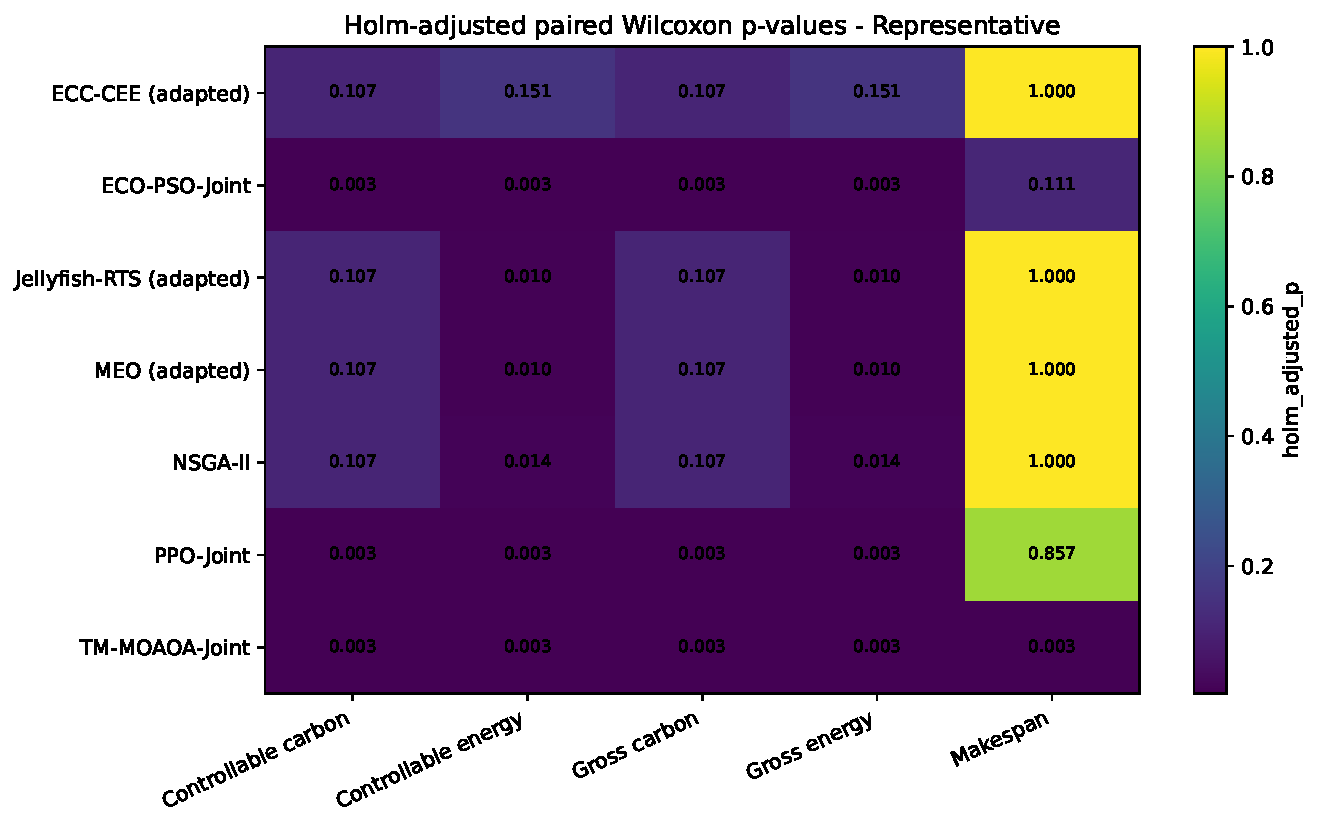
\includegraphics[width=\linewidth]{fig12_holm_pvalues_representative.pdf}
\caption{Representative Holm-adjusted $p$ values.}
\end{subfigure}\hfill
\begin{subfigure}[t]{0.49\textwidth}
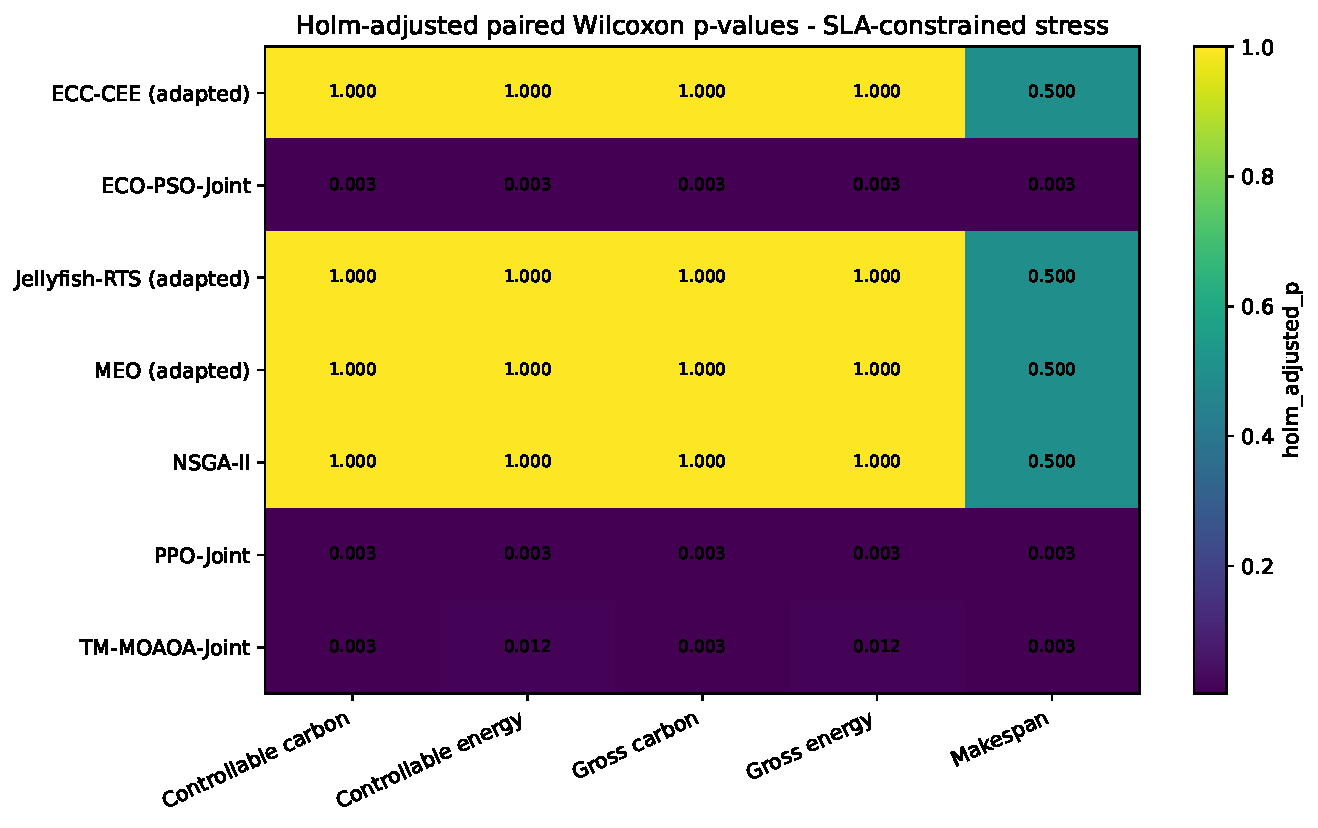
\includegraphics[width=\linewidth]{fig12_holm_pvalues_sla_stress.pdf}
\caption{SLA Holm-adjusted $p$ values.}
\end{subfigure}
\caption{Paired Wilcoxon tests after Holm correction. Scenario/workload cells, not search seeds, form the paired samples.}
\label{fig:significance}
\end{figure*}

\subsection{Runtime and decision overhead}
\label{sec:runtime-results}

Equal objective-call budgets do not imply equal wall-clock cost because each optimizer performs different search bookkeeping. On representative scenarios, \method has a median decision time of \SI{9.08}{s}. The fastest classical competitors are around 5.65--\SI{6.14}{s}, giving a median \method multiplier of 1.48 and a maximum of 1.68. PPO-Joint is substantially heavier at a \SI{90.56}{s} median. Thus, \method is slower than the simplest classical searches but approximately ten times faster than the PPO baseline in this track.

Under SLA stress, the median \method decision time rises to \SI{50.72}{s}. ECO-PSO and MEO have medians of 17.59 and \SI{18.30}{s}; NSGA-II takes \SI{24.56}{s}; PPO-Joint takes \SI{581.60}{s}. The median multiplier relative to the fastest classical method is 2.92, with a maximum of 3.17 in the most expensive Google stress cell. Figure~\ref{fig:runtime} shows the complete distributions summarized by method.

\begin{figure*}[t]
\centering
\begin{subfigure}[t]{0.49\textwidth}
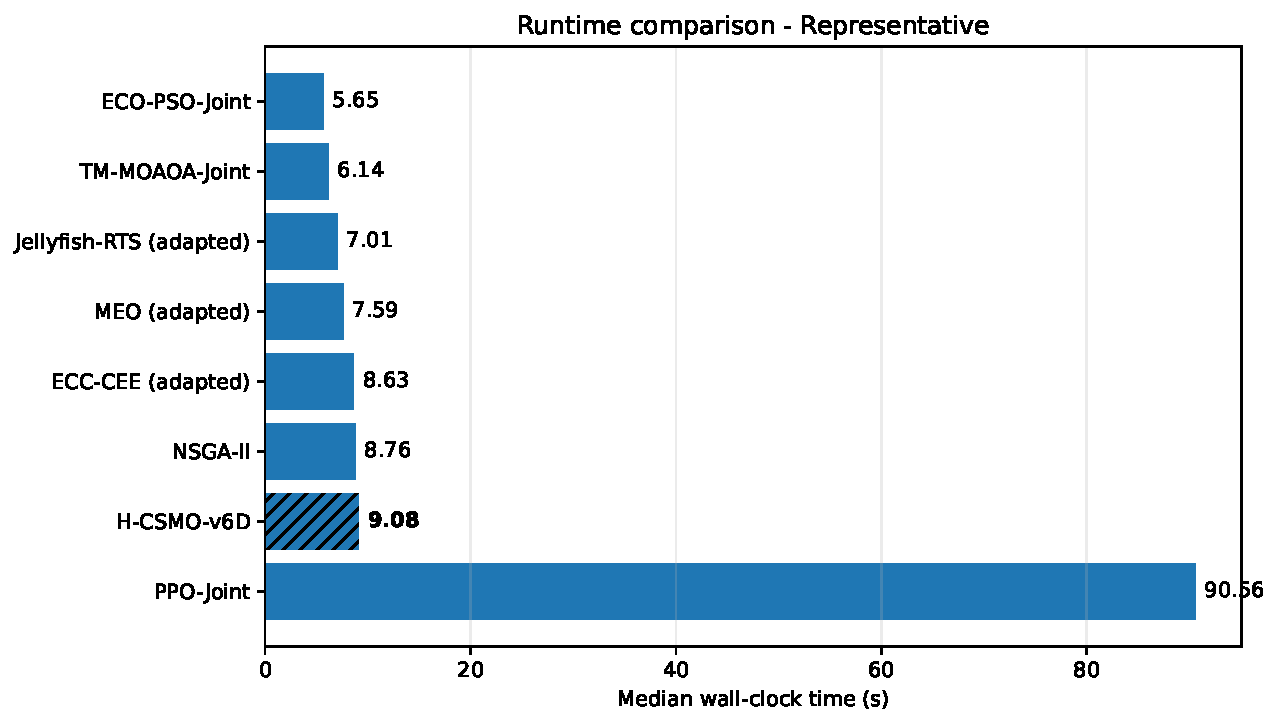
\includegraphics[width=\linewidth]{fig10_runtime_representative.pdf}
\caption{Representative.}
\end{subfigure}\hfill
\begin{subfigure}[t]{0.49\textwidth}
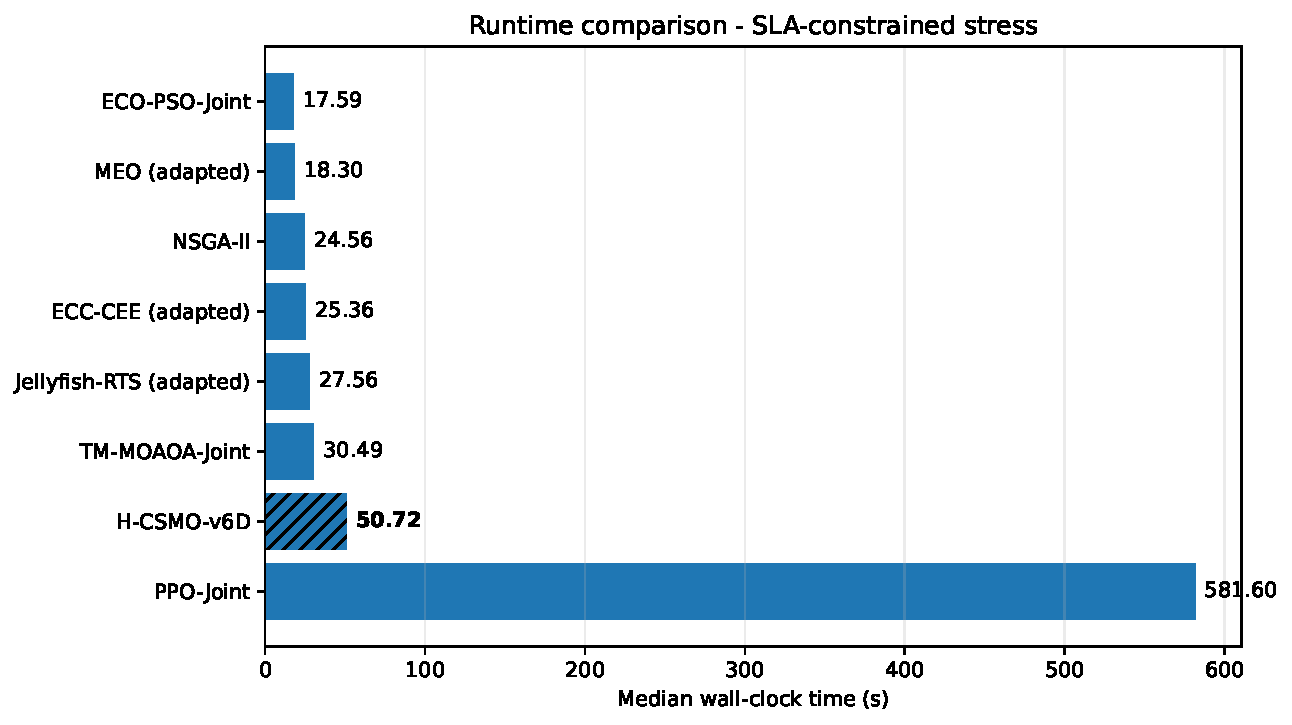
\includegraphics[width=\linewidth]{fig10_runtime_sla_stress.pdf}
\caption{SLA stress.}
\end{subfigure}
\caption{Median wall-clock decision time. The objective-call budget is equal within each scenario; the plot exposes method-specific computational overhead.}
\label{fig:runtime}
\end{figure*}

\subsection{Migration behavior}
\label{sec:migration-results}

Migration remains modest on the representative workloads. For \method, migration energy accounts for a median 0.255\% of gross horizon energy and never exceeds 1.137\%; migration emissions have a median share of 0.317\% and maximum of 0.799\%. The SLA track uses migration more aggressively: median energy and emissions shares are 2.20\% and 1.95\%, while the largest Alibaba stress cases reach 19.97\% and 32.35\%, respectively. These are the cells in which cross-region movement becomes an explicit part of the carbon/latency trade-off rather than a negligible side effect.

The migration-disabled ablation provides the relevant counterfactual. Across the 12 representative ablation cells, the median full-method improvement over migration-disabled scheduling is 99.77\% for controllable carbon, 77.75\% for controllable energy, and 59.35\% for gross energy, while the median makespan difference is below 0.001\%. The high migration fractions observed in a subset of SLA cells are therefore not simply gratuitous movement: the same capability is responsible for large carbon/energy improvements when spatial flexibility matters. Appendix~\ref{app:ablation} reports the complete ablation plots.

\subsection{Ablation and sensitivity}
\label{sec:ablation-results}

The representative-track ablation identifies migration as the largest measured contributor in the median. Other components are more conditional. Median changes from removing adaptive active-pool control or critical-tail repair are close to zero, and the median selected point is unchanged when carbon shifting or the legacy guard is disabled. This does not imply that those mechanisms are redundant: they are protection and regime-selection operators whose effect is triggered only when the archive contains a candidate that crosses the relevant boundary.

The DVFS ablation exposes a different trade-off. Across the representative ablation cells, removing five-state DVFS has a median 5.97\% lower controllable energy and 2.02\% lower controllable carbon than the full method, but a 0.339\% higher makespan. In other words, the full controller uses the extra DVFS range to purchase a shorter critical tail at a small energy/carbon cost rather than treating DVFS as an unconditional energy-saving device. Sensitivity plots show the same mechanism: restricted balanced/eco policies can reduce energy, while the full five-state policy reaches the lower makespan operating point. Across all sensitivity settings, deadline-miss ratio remains zero.
% ---- END sections/07_results.tex ----
% ---- BEGIN sections/08_discussion.tex ----
\section{Discussion}
\label{sec:discussion}

\subsection{Why the Pareto result is stronger than universal single-metric claims}

The full benchmark separates two questions that are often conflated in multi-objective scheduling: whether a method produces a strong \emph{operating point}, and whether it produces a strong \emph{set of alternatives}. On representative workloads, \method performs well under both views: it has the best overall single-profile rank and the best hypervolume. Under SLA stress, the two views separate. NSGA-II has the better average rank for the selected balanced schedules, largely because it more often reaches the minimum-energy point. \method nevertheless has the highest three-objective hypervolume in every stress cell and the best average makespan rank. This means that its archive covers a broader useful carbon--energy--latency region even when another method supplies the lowest value of one individual metric.

This distinction matters operationally. A scheduler deployed under a carbon budget, an energy cap, or a latency objective may prefer different points from the same Pareto set. Reporting only the balanced profile would hide that flexibility; reporting only hypervolume would hide the workload-specific regressions of the selected profile. The two views together provide a more faithful description of what the method offers.

\subsection{Sparse-regime behavior and active-pool control}

The four representative cells that are most difficult for \method are all 30-task scenarios. At that scale, the infrastructure has substantial capacity relative to demand, and a specialist strategy can consolidate aggressively onto one or two highly efficient nodes. \method deliberately evaluates multiple profile pools and retains headroom for latency and carbon shifts. The additional active capacity can therefore be unnecessary in the sparsest cells, especially when the strongest competitor happens to select an energy-specialized constructor.

The workload-pressure estimator in Eq.~\eqref{eq:pool-size} reduces this effect by allowing one-node pools, and the protected selector prevents large makespan regressions. The remaining gaps show that sparse-regime scheduling is not simply a smaller version of the contention problem: activation cost dominates sooner than queueing cost. For this reason, the representative results are reported separately by task scale and the heatmap remains part of the main evaluation.

\subsection{Interpreting controllable and gross carbon/energy}

The two-layer accounting changes how percentage improvements should be read. A 20\% change in scheduler-controllable energy can become a sub-percent change in gross fixed-horizon energy when the infrastructure floor dominates the horizon. This is not a contradiction. $E_{\mathrm{ctrl}}$ measures the part affected by placement, timing, DVFS, sleep/wake, and migration; $E_{\mathrm{gross}}$ answers the facility-level question after restoring the fixed background floor. The same relation holds for carbon.

The representative track illustrates this directly: median controllable-carbon improvement versus the strongest per-cell competitor is 21.99\%, while median gross-carbon improvement is 0.39\%. Presenting only the controllable metric would overstate the facility-level impact; presenting only the gross metric would make meaningful scheduler differences look negligible. Both layers are therefore necessary for a carbon-aware scheduling study.

\subsection{Migration as an active control rather than a free benefit}

Migration is beneficial only when the destination advantage exceeds transfer overhead. The representative workloads stay in a regime where that overhead is small. Several Alibaba SLA cells are different: cross-region movement contributes a visibly larger fraction of energy and emissions. The migration-disabled ablation shows why the full method still chooses those moves. Removing migration collapses the scheduler's spatial flexibility and produces much larger carbon and energy values in the diagnostic case. The practical conclusion is not that migration is cheap, but that it is a controlled resource that should be charged explicitly and used where its benefit is measurable.

\subsection{Deployment regime and decision time}

The wall-clock results place \method between classical metaheuristics and the PPO baseline. Its structured constructors, archive handling, and tail analysis are more expensive than ECO-PSO or MEO, but the method remains roughly an order of magnitude faster than PPO in both tracks. On the representative workloads, median decision time is approximately nine seconds. The SLA track reaches about 51 seconds because each scenario has 150 tasks and a 396-call budget. Such times fit rolling/batch rescheduling more naturally than sub-second per-request dispatch. For tighter online loops, the same architecture can be used with a smaller call budget; the sensitivity experiment shows that reducing the budget to 60--80\% preserves the selected point in the tested scenario while lowering runtime.

\subsection{Evaluation scope and transferability}

The evidence is based on trace-derived simulation with an explicit external power/network/carbon model, not on measurements from a production edge--cloud deployment. The simulator exposes the same controls and repair semantics to every compared method, and all reported schedules were replayed from saved decision vectors, but real platforms can introduce effects not represented here, including interference, uncertain transfer throughput, inaccurate carbon forecasts, and hardware-specific DVFS transition costs. The three adapted baselines are therefore labeled as adapted implementations, and the SLA arrival permutations are described as controlled workload-seed replications rather than untouched trace samples.

These boundaries do not alter the comparative results inside the declared model; they define the next validation step. A deployment study should preserve the same distinction between controllable and gross energy, measure migration traffic directly, and test whether the protected tail selector remains stable when service-time and carbon forecasts are noisy.
% ---- END sections/08_discussion.tex ----
% ---- BEGIN sections/09_conclusion.tex ----
\section{Conclusion}
\label{sec:conclusion}

This paper presented \method, a guarded multi-profile scheduler for multi-region edge--cloud systems with joint node placement, temporal shifting, five-state DVFS, migration, sleep/wake control, and time-varying regional carbon intensity. The method combines structured profile constructors, workload-adaptive active pools, equal-budget stochastic refinement, and a protected critical-tail stage that can accelerate the latest-finishing tasks only inside fixed carbon, energy, gross-accounting, and makespan guards. A two-layer accounting model separates scheduler-controllable energy and emissions from the fixed infrastructure floor while retaining gross fixed-horizon results.

Across 12 frozen representative scenarios, \method achieved the best overall average rank among eight equal-budget methods (1.98/8), including the best average rank for all five primary metrics. Its exact normalized carbon--energy--makespan hypervolume ranked first in every representative scenario. Under 12 SLA-constrained workload-seed stress scenarios, NSGA-II obtained the best overall single-profile rank, while \method ranked second (2.64/8), retained the best average makespan rank, and reduced median controllable carbon by 12.95\% relative to the strongest per-cell competitor. The \method Pareto set achieved the highest normalized three-objective hypervolume in all 24 evaluated scenarios. Paired Wilcoxon tests with Holm correction further showed significant advantages over ECO-PSO, TM-MOAOA, and PPO across all five primary SLA metrics.

The results indicate that the most reliable advantage of \method is not universal domination of every metric, but the quality of the protected multi-objective operating region it exposes. Future work will transfer the same frozen decision logic to a hardware-backed edge--cloud testbed, incorporate forecast uncertainty directly into candidate scoring, and investigate lower-cost archive updates for sub-second or few-second decision cycles.
% ---- END sections/09_conclusion.tex ----
% ---- BEGIN sections/10_appendix.tex ----
\appendix

\section{Additional Distributions and Convergence}
\label{app:distributions}

Figures~\ref{fig:box-carbon}--\ref{fig:box-makespan} report per-scenario normalized distributions for the five primary metrics. These plots complement average ranks by exposing dispersion and outliers. Figure~\ref{fig:convergence} shows median best balanced utility as the objective-call budget is consumed.

\begin{figure*}[p]
\centering
\begin{subfigure}{0.49\textwidth}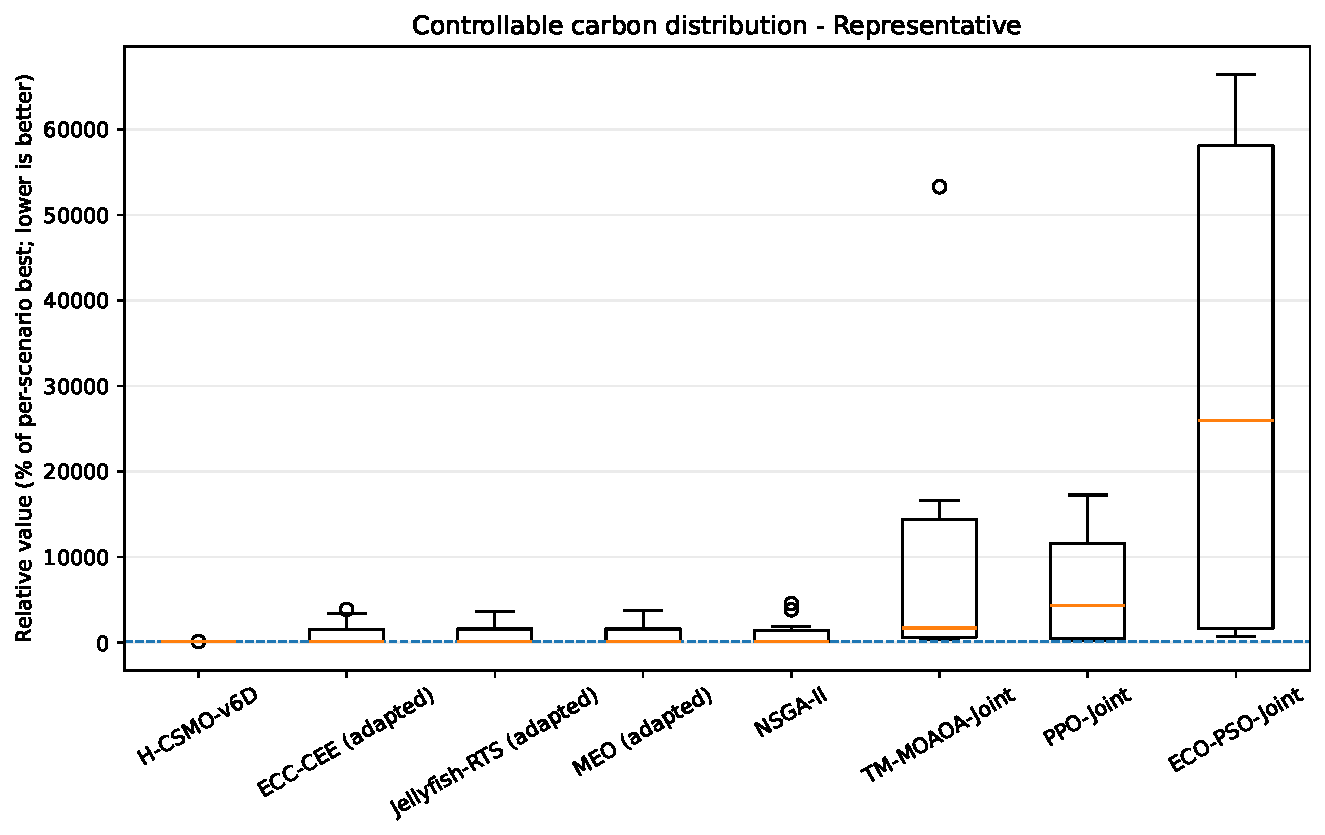
\includegraphics[width=\linewidth]{fig04_representative_scheduler_controllable_emissions_g_boxplot.pdf}\caption{Representative.}\end{subfigure}\hfill
\begin{subfigure}{0.49\textwidth}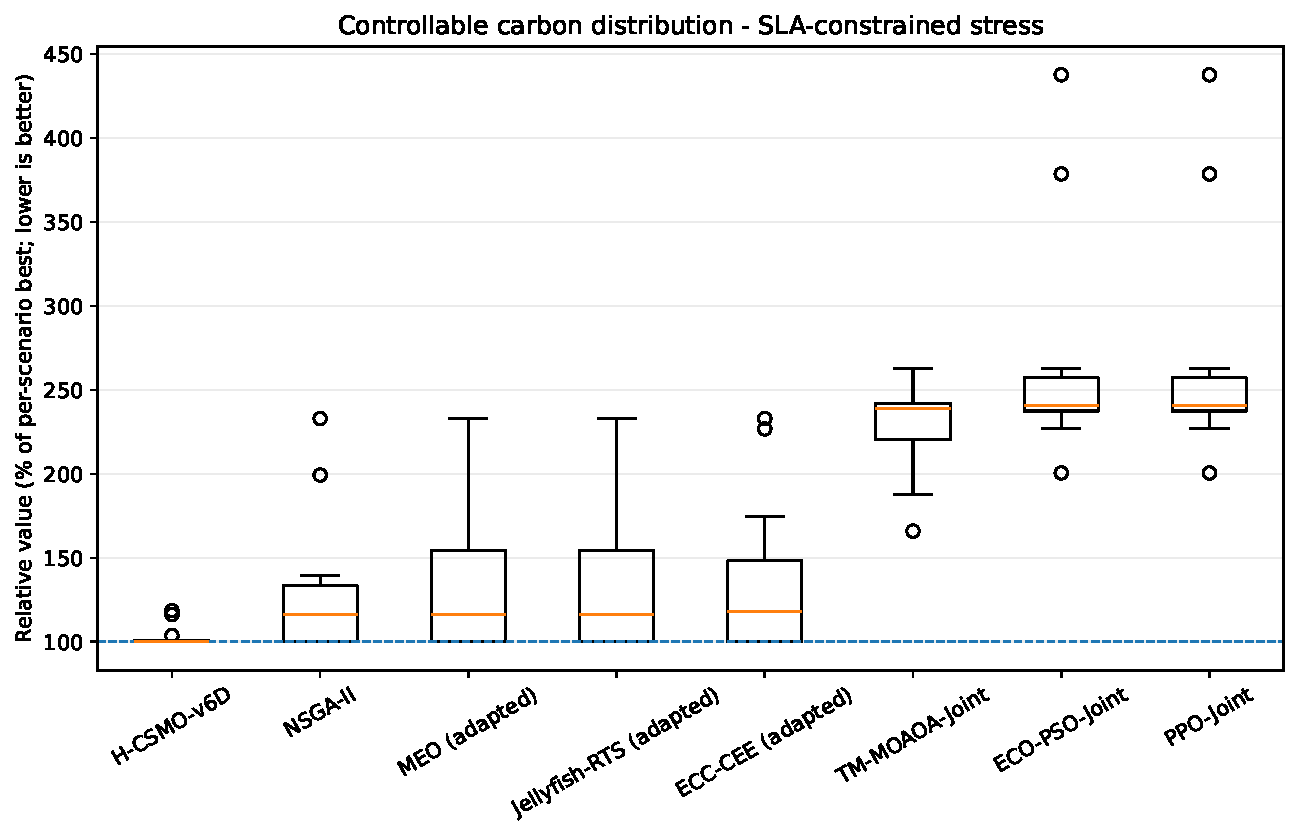
\includegraphics[width=\linewidth]{fig04_sla_stress_scheduler_controllable_emissions_g_boxplot.pdf}\caption{SLA stress.}\end{subfigure}
\caption{Controllable-carbon distribution relative to the best method in each scenario.}\label{fig:box-carbon}
\end{figure*}

\begin{figure*}[p]
\centering
\begin{subfigure}{0.49\textwidth}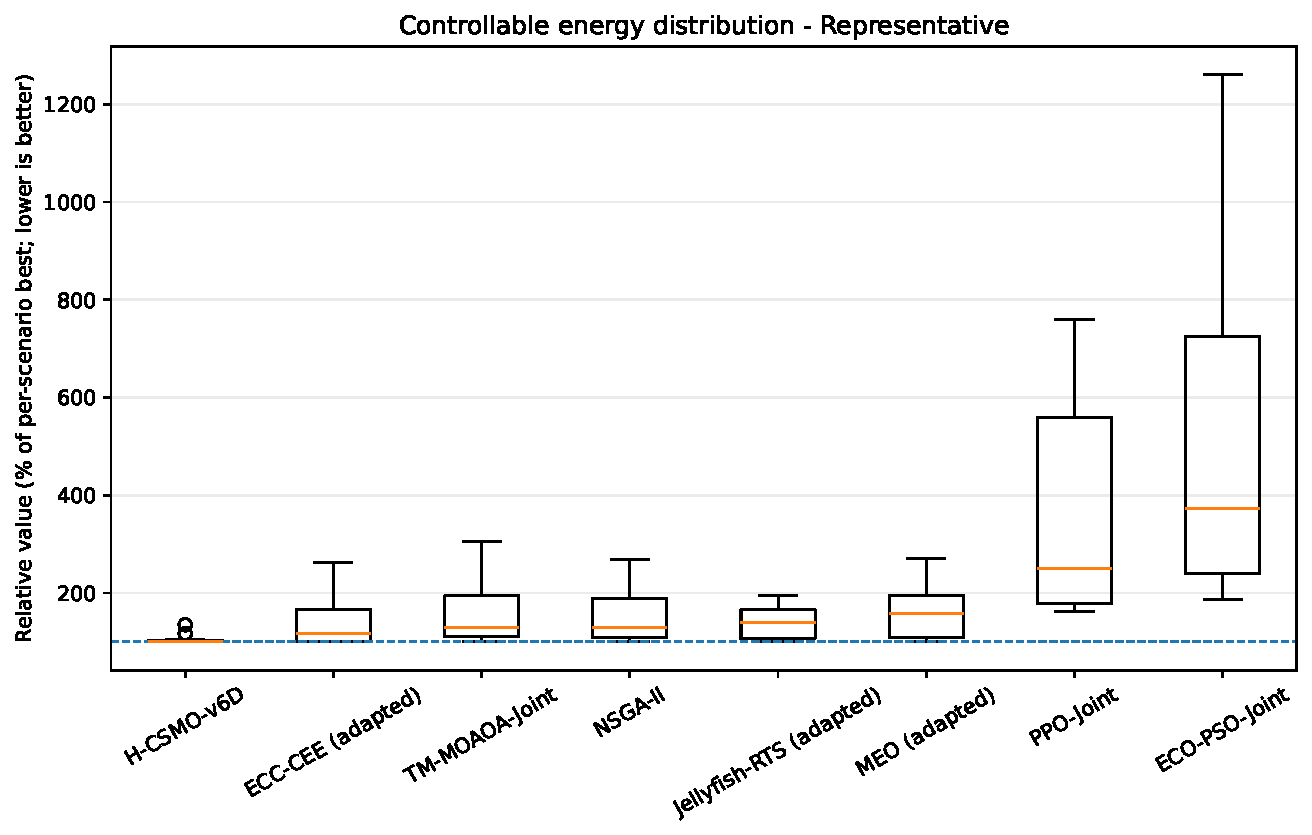
\includegraphics[width=\linewidth]{fig05_representative_scheduler_controllable_energy_wh_boxplot.pdf}\caption{Representative.}\end{subfigure}\hfill
\begin{subfigure}{0.49\textwidth}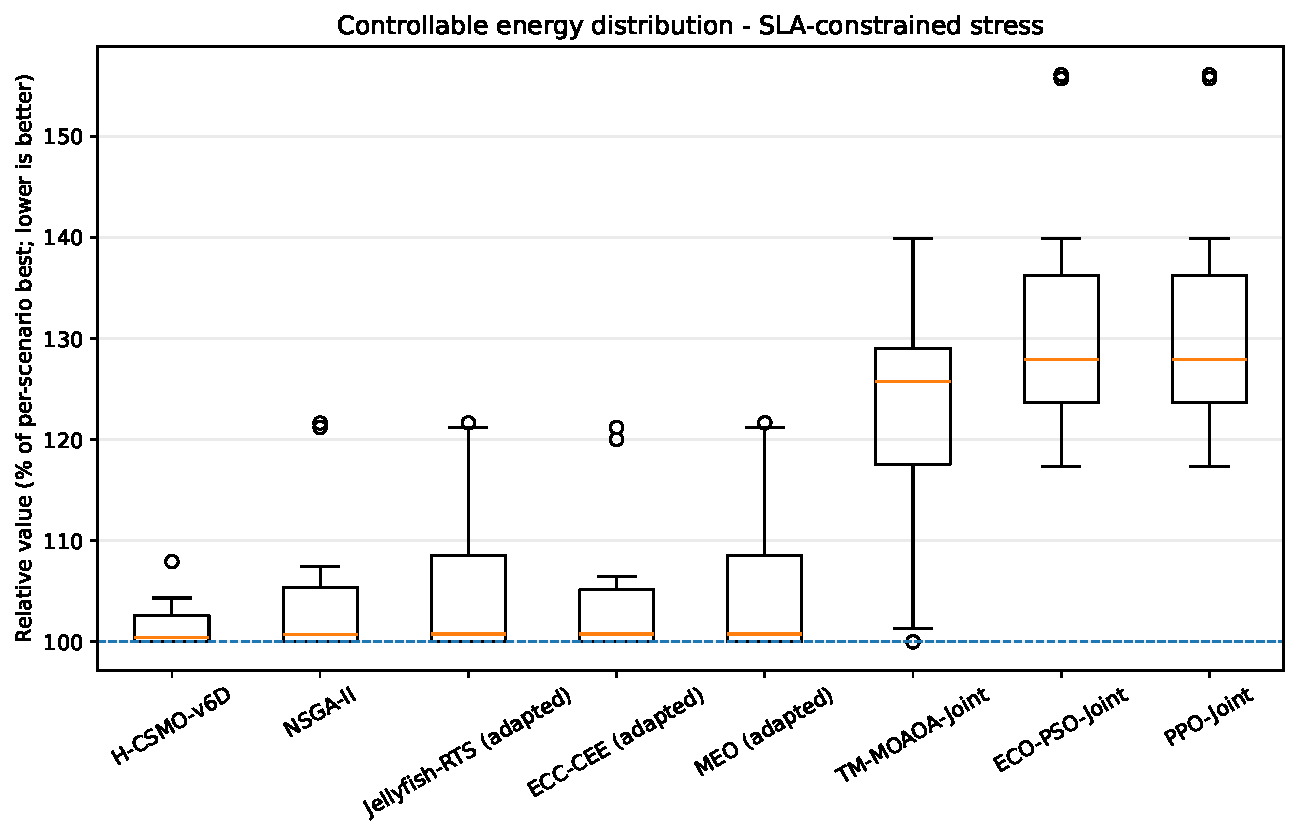
\includegraphics[width=\linewidth]{fig05_sla_stress_scheduler_controllable_energy_wh_boxplot.pdf}\caption{SLA stress.}\end{subfigure}
\caption{Controllable-energy distribution relative to the best method in each scenario.}\label{fig:box-energy}
\end{figure*}

\begin{figure*}[p]
\centering
\begin{subfigure}{0.49\textwidth}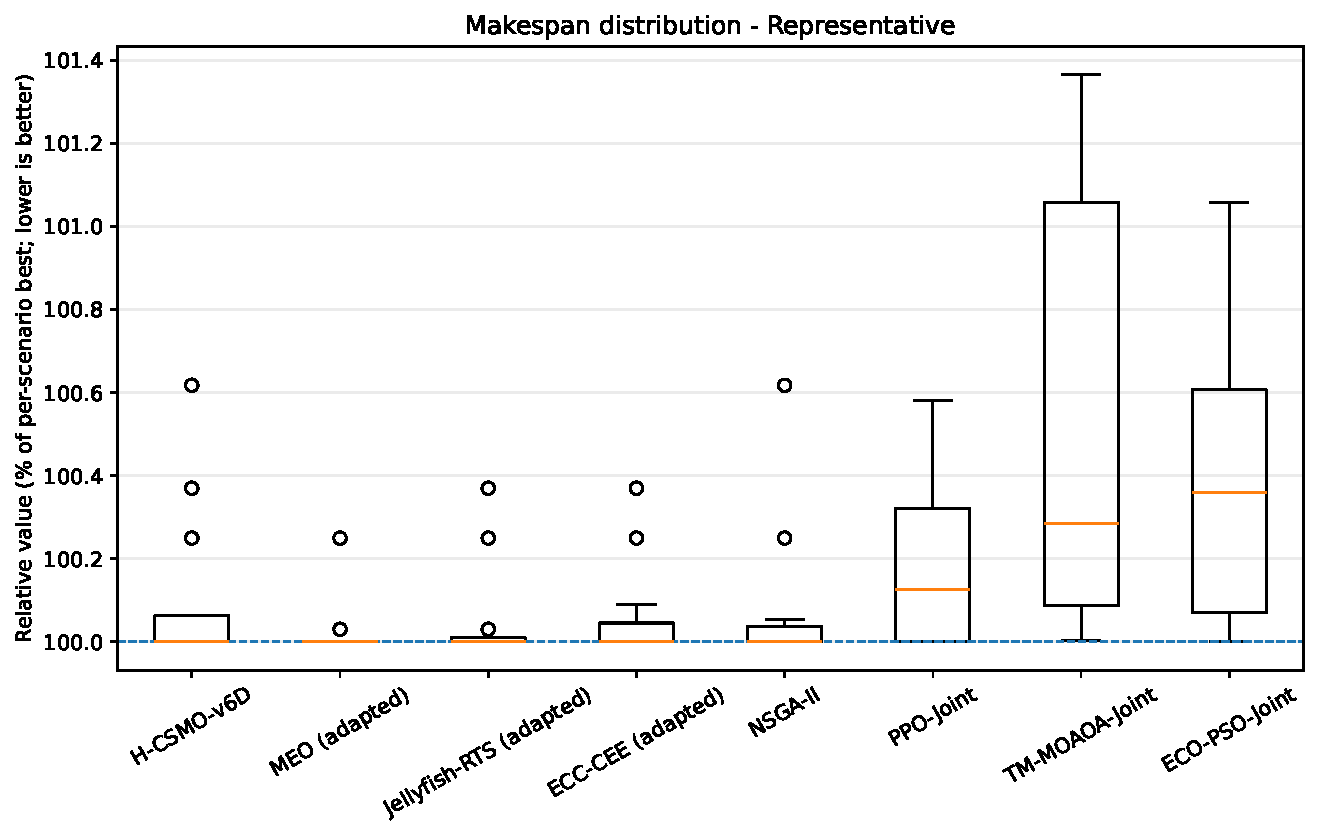
\includegraphics[width=\linewidth]{fig08_representative_makespan_s_boxplot.pdf}\caption{Representative.}\end{subfigure}\hfill
\begin{subfigure}{0.49\textwidth}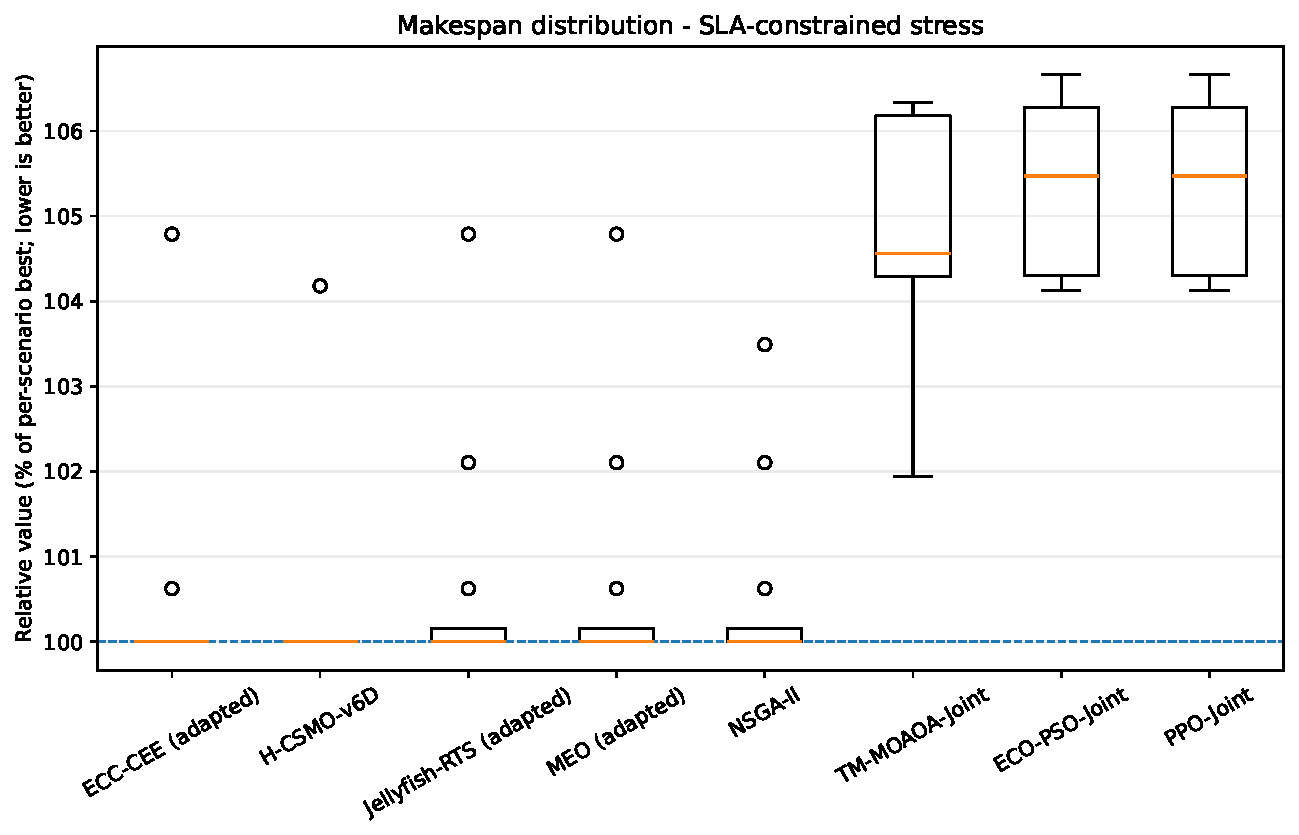
\includegraphics[width=\linewidth]{fig08_sla_stress_makespan_s_boxplot.pdf}\caption{SLA stress.}\end{subfigure}
\caption{Makespan distribution relative to the best method in each scenario.}\label{fig:box-makespan}
\end{figure*}

\begin{figure*}[p]
\centering
\begin{subfigure}{0.49\textwidth}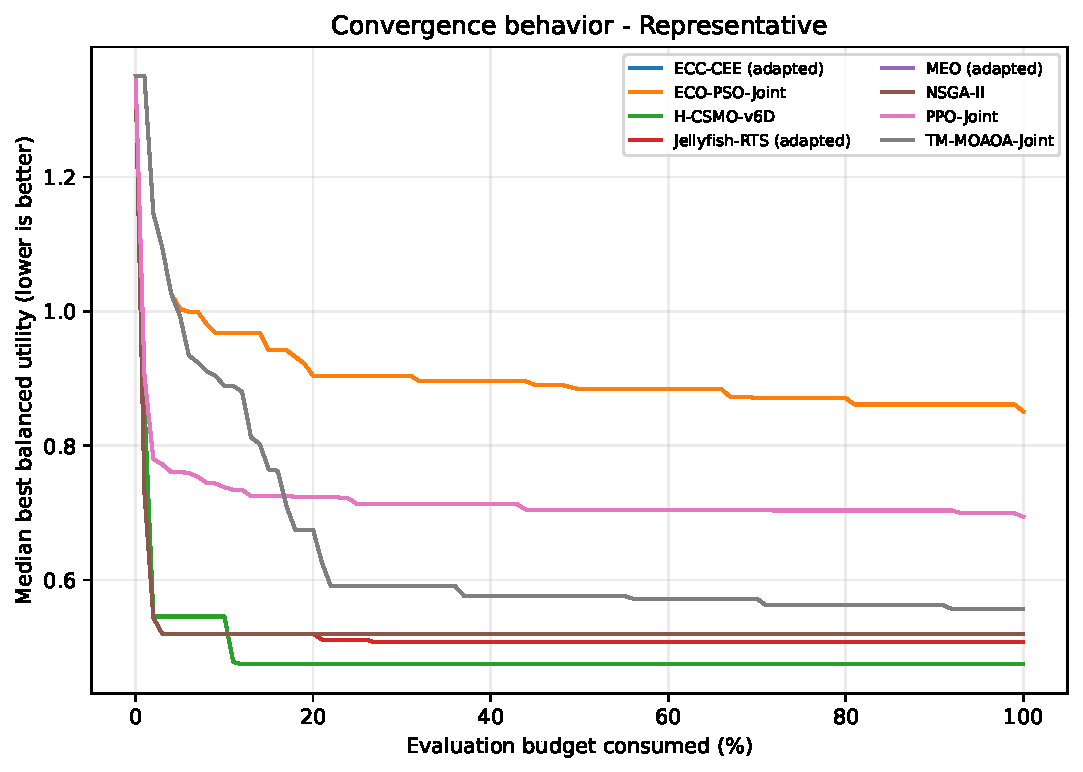
\includegraphics[width=\linewidth]{fig15_convergence_representative.pdf}\caption{Representative.}\end{subfigure}\hfill
\begin{subfigure}{0.49\textwidth}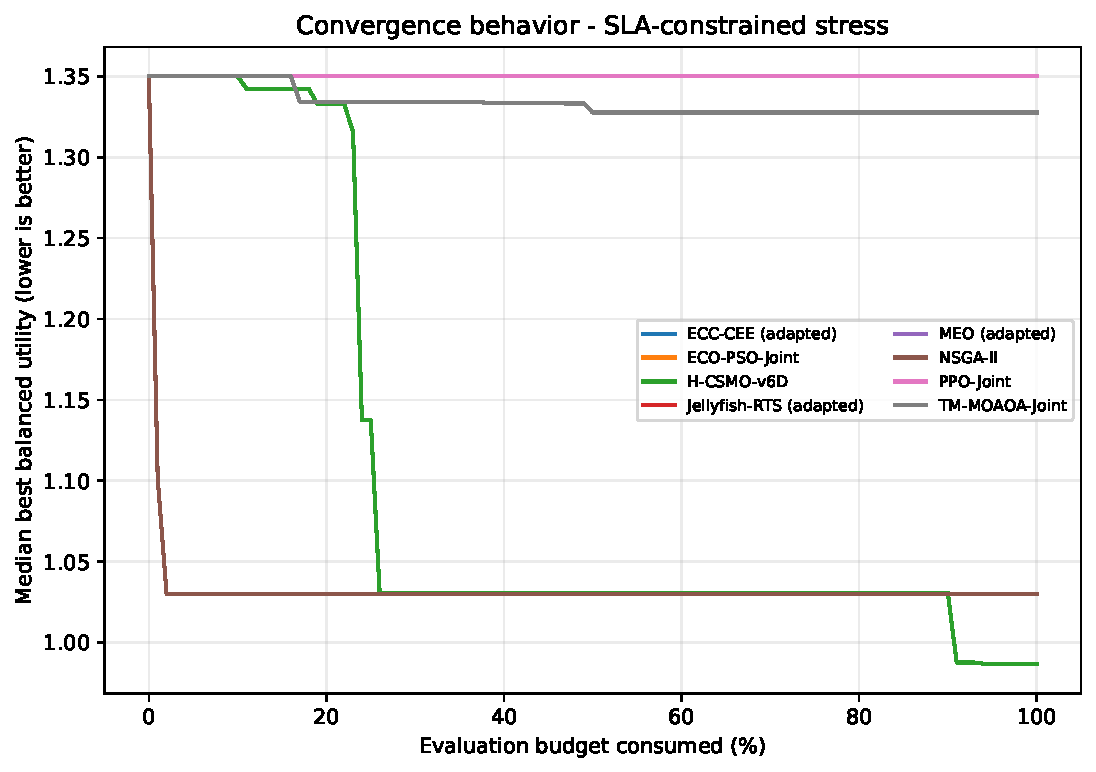
\includegraphics[width=\linewidth]{fig15_convergence_sla_stress.pdf}\caption{SLA stress.}\end{subfigure}
\caption{Median convergence of the best balanced utility as a function of the consumed evaluation budget.}\label{fig:convergence}
\end{figure*}

\section{Ablation Study}
\label{app:ablation}

The equal-budget ablations remove one control from the full method while keeping the shared evaluator and objective-call budget unchanged. Figures~\ref{fig:ablation-carbon} and \ref{fig:ablation-energy-time} report the full-method improvement relative to each ablation. Positive values favor the full scheduler. Constructor-only and historical-v3C entries are diagnostic references and are not equal-budget architectural ablations.

\begin{figure*}[p]
\centering
\begin{subfigure}{0.49\textwidth}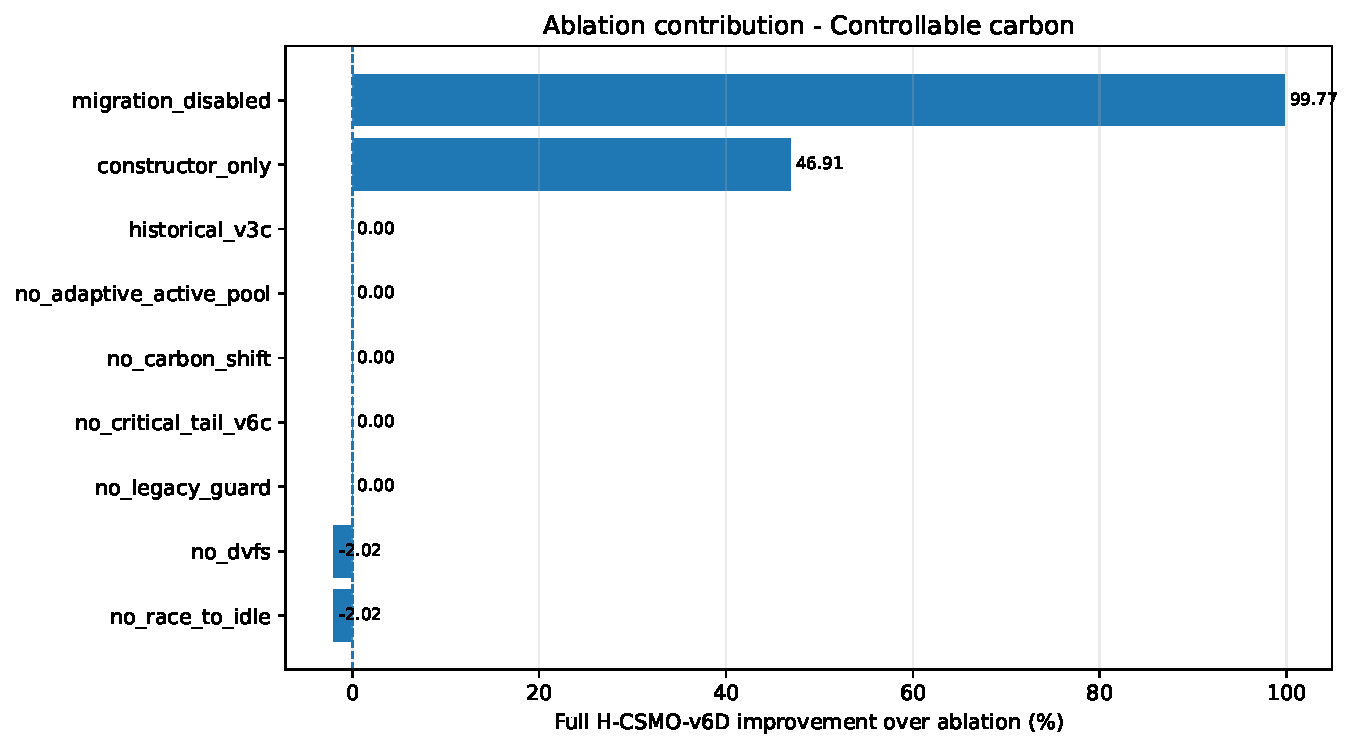
\includegraphics[width=\linewidth]{fig18_ablation_full_improvement_controllable_carbon_pct.pdf}\caption{Controllable carbon.}\end{subfigure}\hfill
\begin{subfigure}{0.49\textwidth}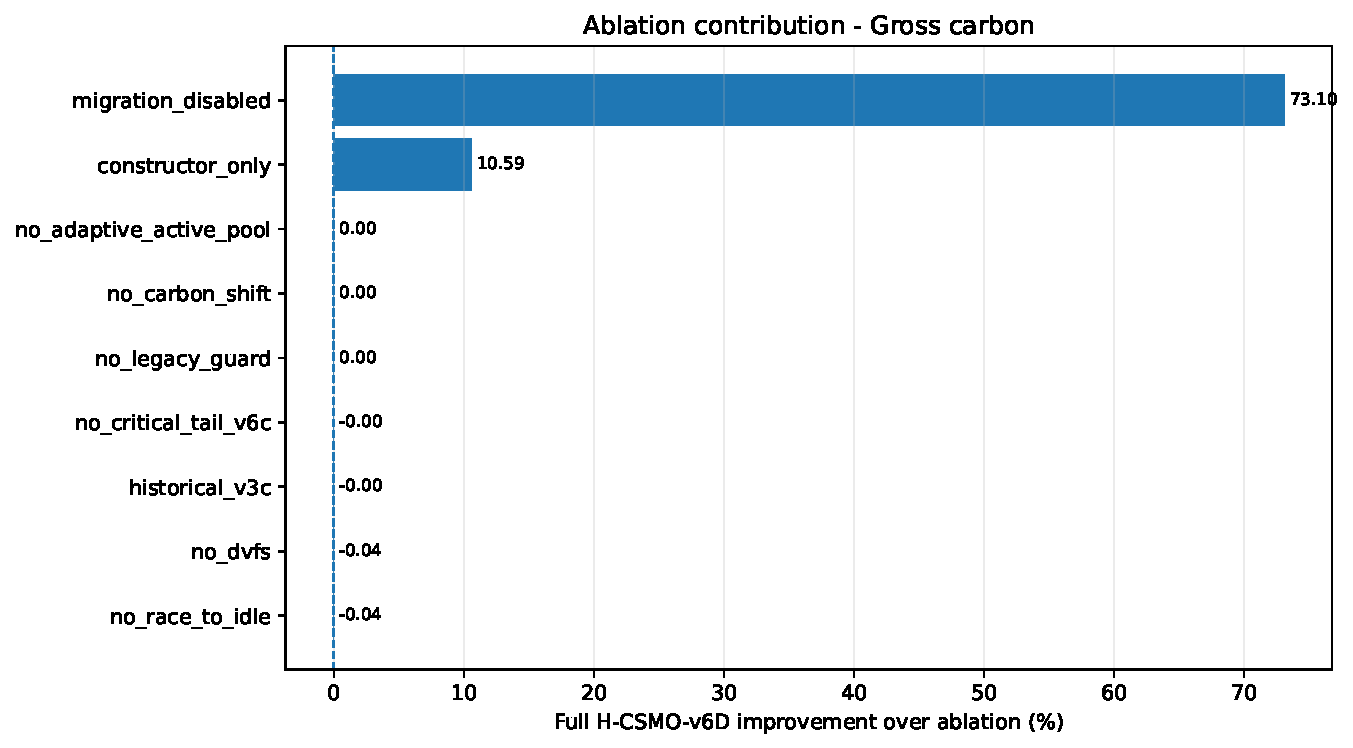
\includegraphics[width=\linewidth]{fig20_ablation_full_improvement_gross_carbon_pct.pdf}\caption{Gross carbon.}\end{subfigure}
\caption{Ablation results for carbon metrics.}\label{fig:ablation-carbon}
\end{figure*}

\begin{figure*}[p]
\centering
\begin{subfigure}{0.33\textwidth}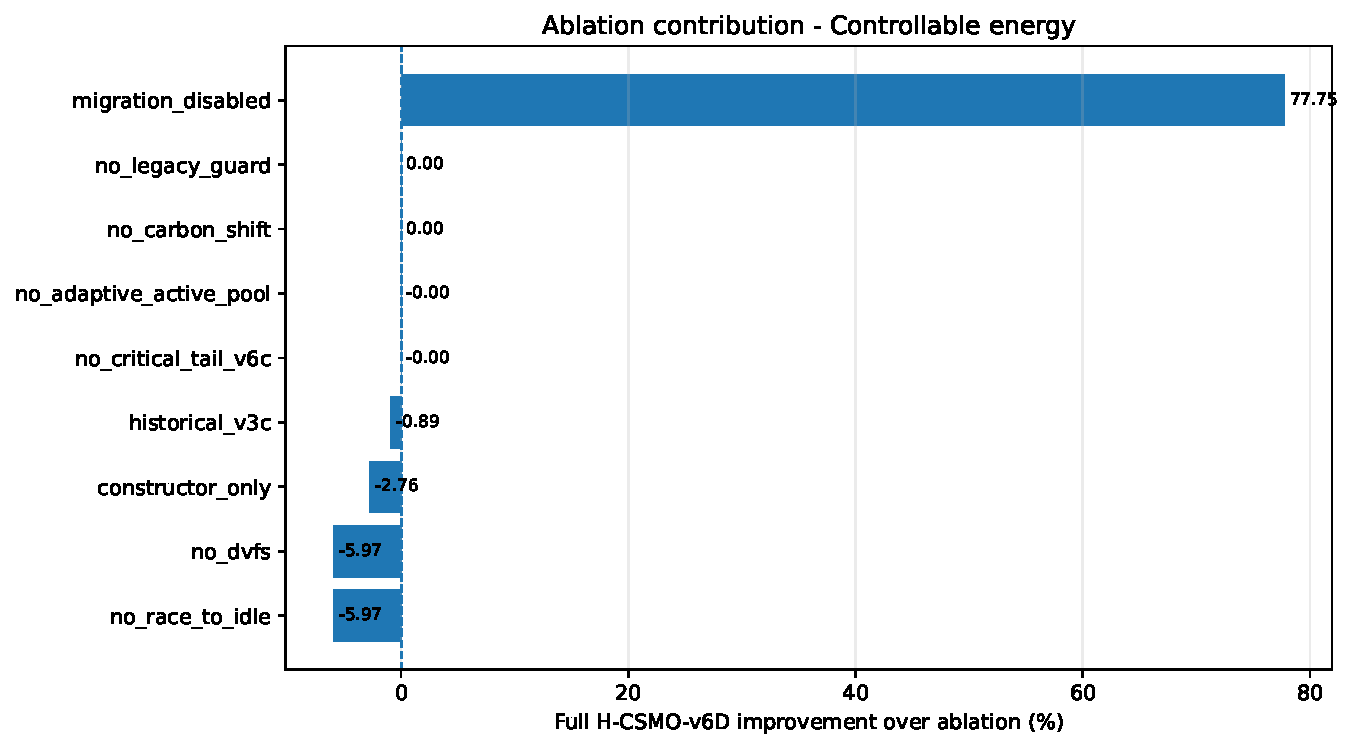
\includegraphics[width=\linewidth]{fig19_ablation_full_improvement_controllable_energy_pct.pdf}\caption{Controllable energy.}\end{subfigure}
\begin{subfigure}{0.33\textwidth}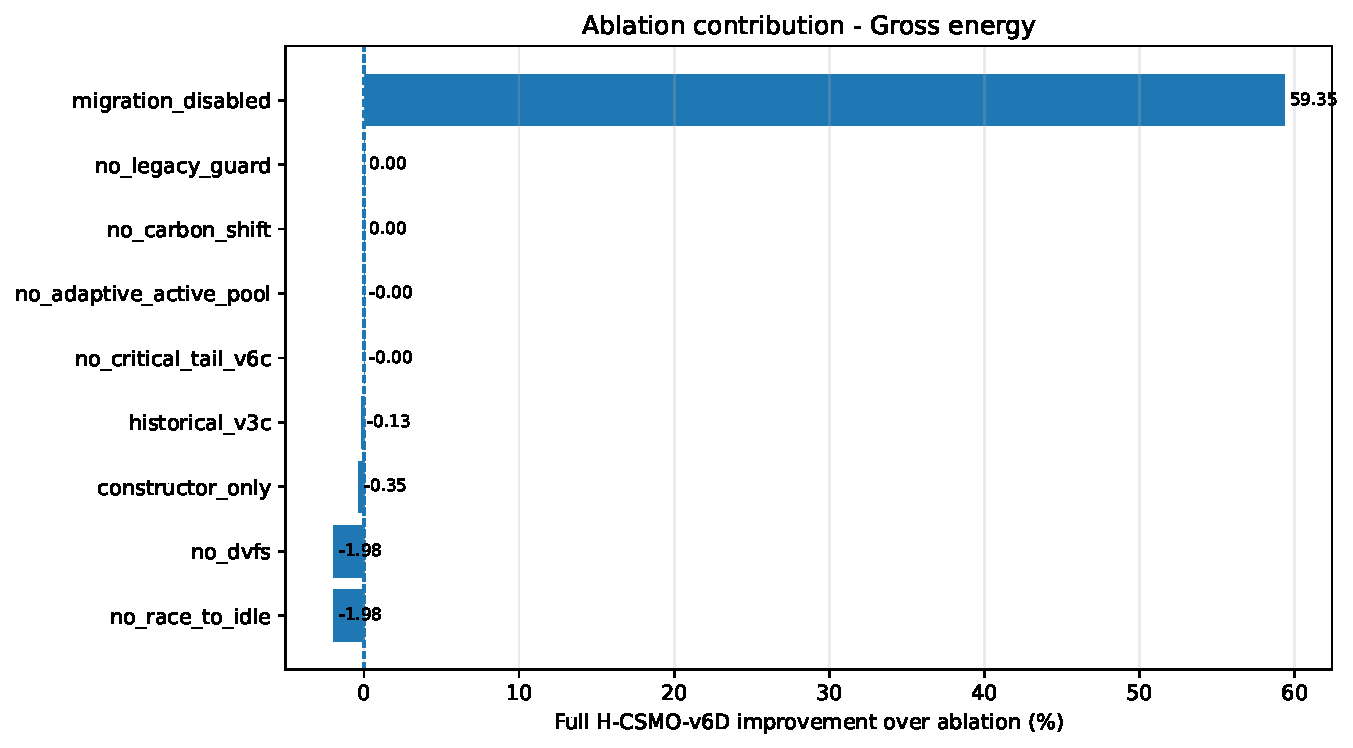
\includegraphics[width=\linewidth]{fig21_ablation_full_improvement_gross_energy_pct.pdf}\caption{Gross energy.}\end{subfigure}
\begin{subfigure}{0.33\textwidth}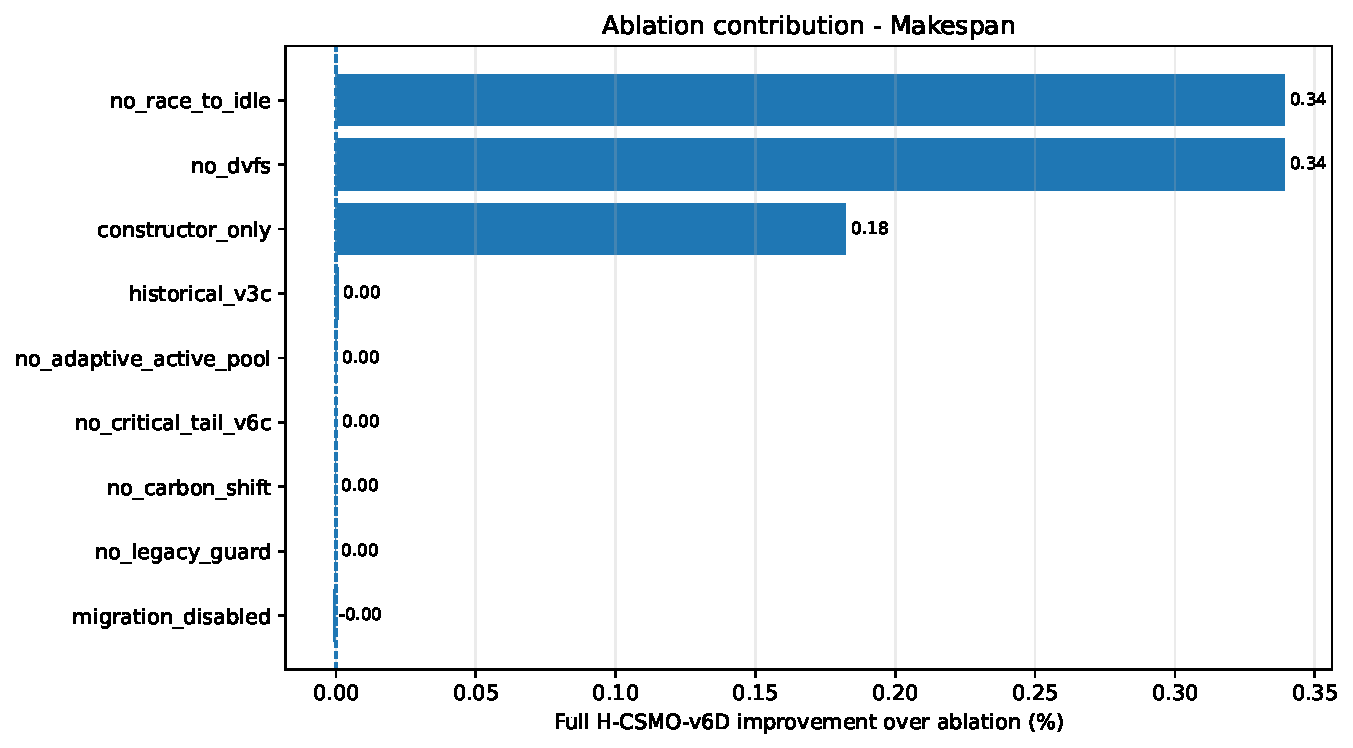
\includegraphics[width=\linewidth]{fig22_ablation_full_improvement_makespan_pct.pdf}\caption{Makespan.}\end{subfigure}
\caption{Ablation results for energy and makespan.}\label{fig:ablation-energy-time}
\end{figure*}

\section{Sensitivity Analysis}
\label{app:sensitivity}

Sensitivity is evaluated only for controls active in the frozen implementation. Figure~\ref{fig:sensitivity-primary} shows the most consequential families: active-pool size, critical-tail size, DVFS policy, and evaluation budget. Guard thresholds and migration/carbon-shift settings are provided in the artifact package and summarized by Fig.~\ref{fig:sensitivity-guards}. Deadline-miss ratio remains zero for all tested settings.

\begin{figure*}[p]
\centering
\begin{subfigure}{0.49\textwidth}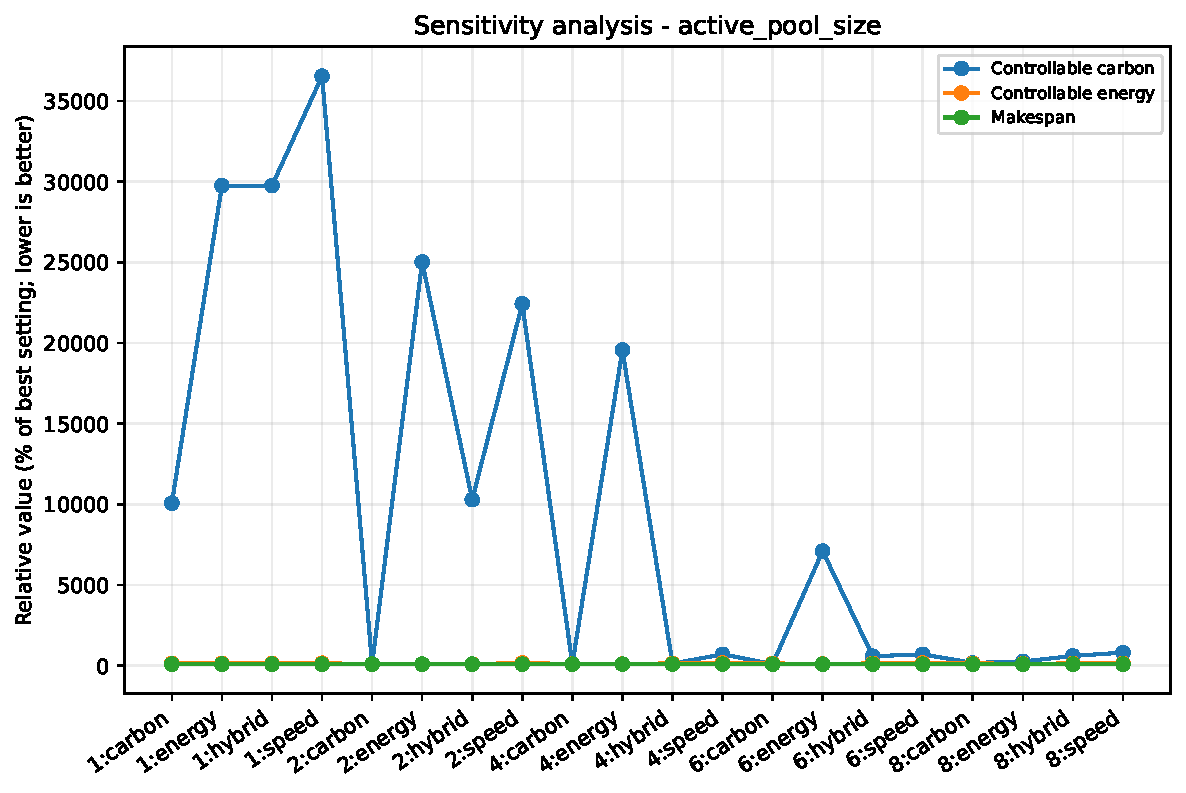
\includegraphics[width=\linewidth]{fig23_sensitivity_active_pool_size.pdf}\caption{Active-pool size.}\end{subfigure}\hfill
\begin{subfigure}{0.49\textwidth}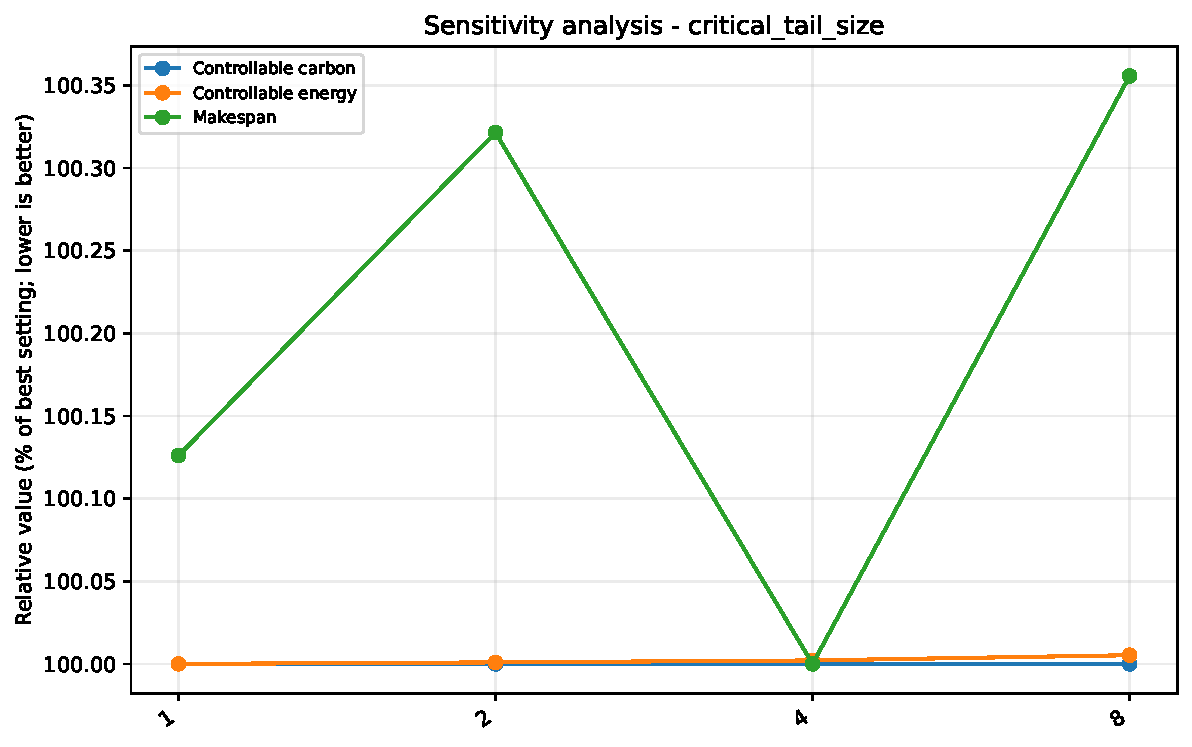
\includegraphics[width=\linewidth]{fig26_sensitivity_critical_tail_size.pdf}\caption{Critical-tail size.}\end{subfigure}
\vspace{2mm}
\begin{subfigure}{0.49\textwidth}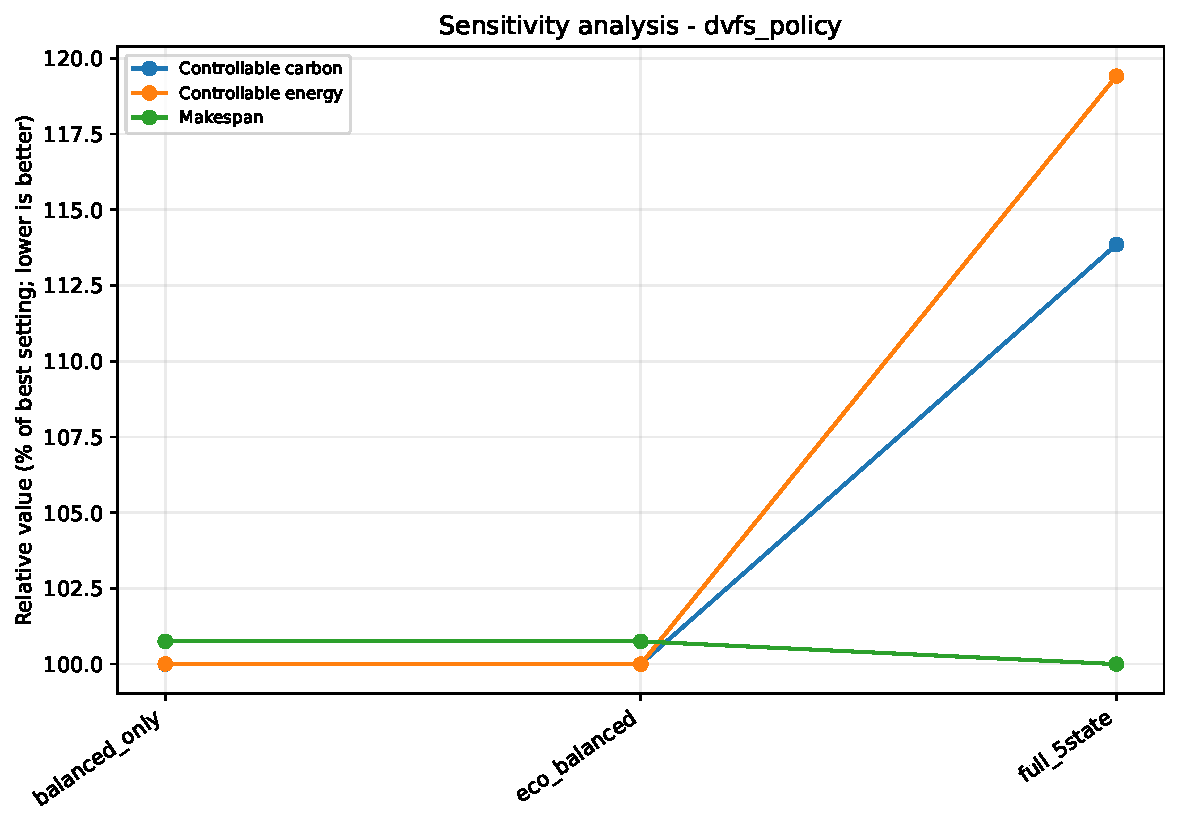
\includegraphics[width=\linewidth]{fig27_sensitivity_dvfs_policy.pdf}\caption{DVFS policy.}\end{subfigure}\hfill
\begin{subfigure}{0.49\textwidth}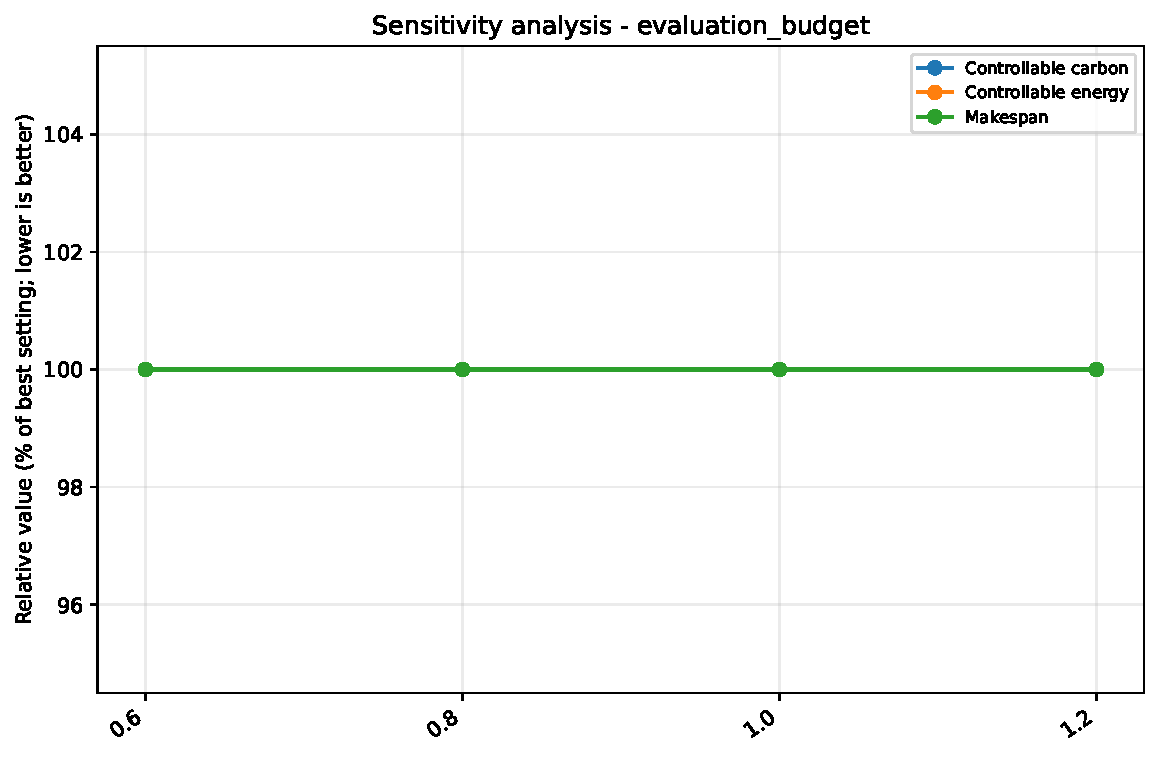
\includegraphics[width=\linewidth]{fig28_sensitivity_evaluation_budget.pdf}\caption{Evaluation budget.}\end{subfigure}
\caption{Sensitivity of active search controls. Lower relative values are better within each metric.}\label{fig:sensitivity-primary}
\end{figure*}

\begin{figure*}[p]
\centering
\begin{subfigure}{0.49\textwidth}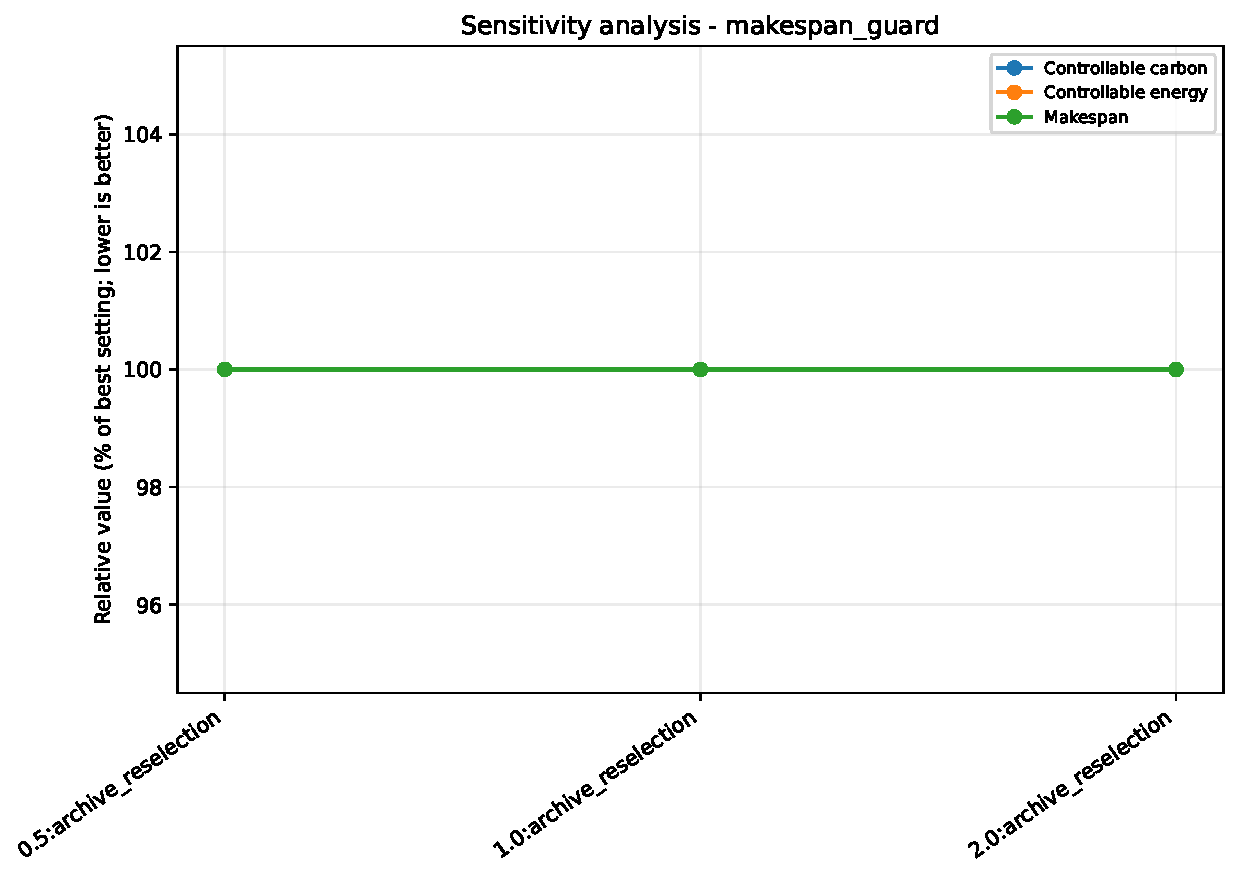
\includegraphics[width=\linewidth]{fig31_sensitivity_makespan_guard.pdf}\caption{Makespan guard.}\end{subfigure}\hfill
\begin{subfigure}{0.49\textwidth}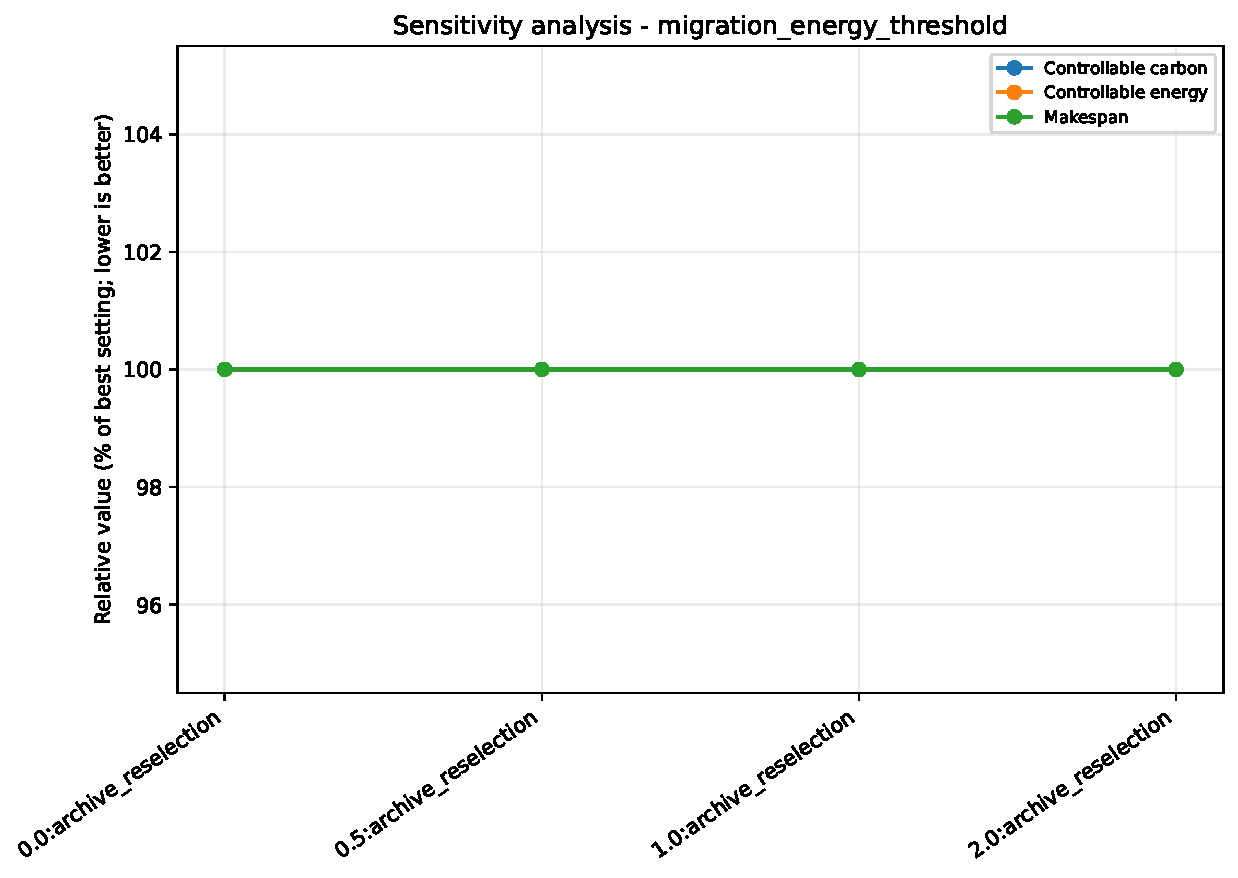
\includegraphics[width=\linewidth]{fig32_sensitivity_migration_energy_threshold.pdf}\caption{Migration-energy threshold.}\end{subfigure}
\caption{Sensitivity of protection controls.}\label{fig:sensitivity-guards}
\end{figure*}

\section{Migration and Operating Profiles}
\label{app:migration}

Figure~\ref{fig:migration-appendix} relates migration-energy share to gross energy. Figure~\ref{fig:profiles-appendix} shows the median carbon--energy locations of the four operating profiles; marker size reflects the makespan component. These plots make explicit that migration and profile choice are active trade-off controls rather than unreported side effects.

\begin{figure*}[p]
\centering
\begin{subfigure}{0.49\textwidth}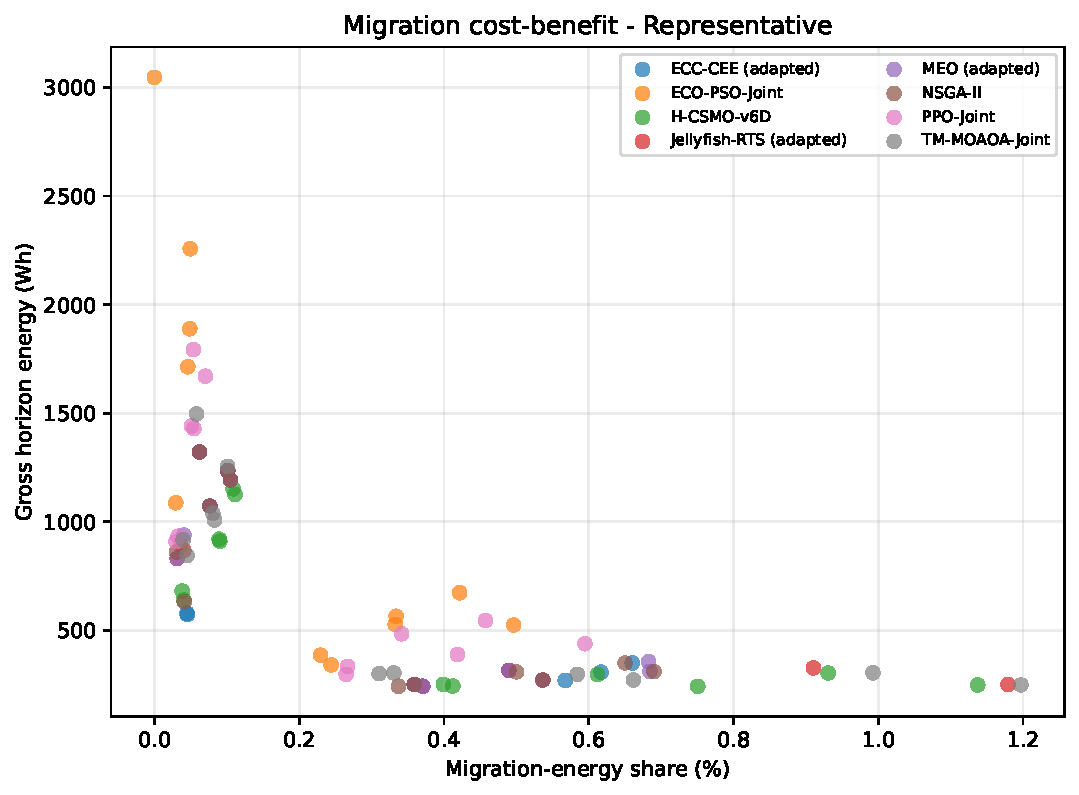
\includegraphics[width=\linewidth]{fig16_migration_cost_benefit_representative.pdf}\caption{Representative.}\end{subfigure}\hfill
\begin{subfigure}{0.49\textwidth}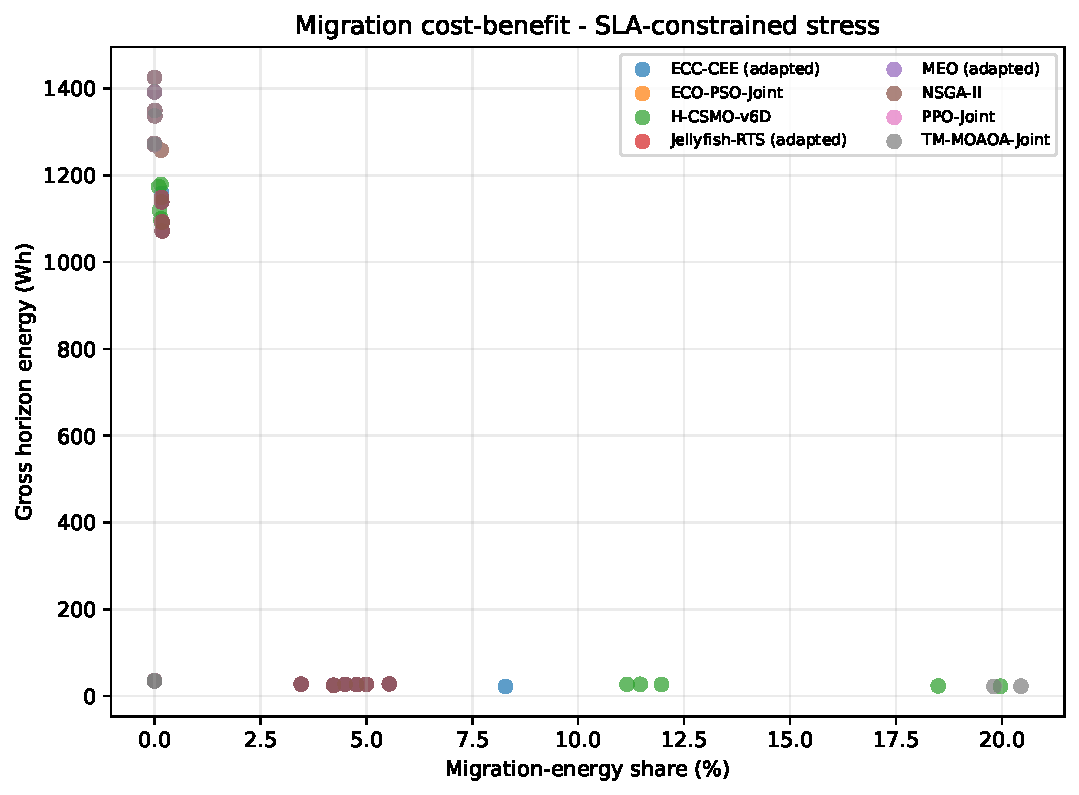
\includegraphics[width=\linewidth]{fig16_migration_cost_benefit_sla_stress.pdf}\caption{SLA stress.}\end{subfigure}
\caption{Migration cost-benefit distributions.}\label{fig:migration-appendix}
\end{figure*}

\begin{figure*}[p]
\centering
\begin{subfigure}{0.49\textwidth}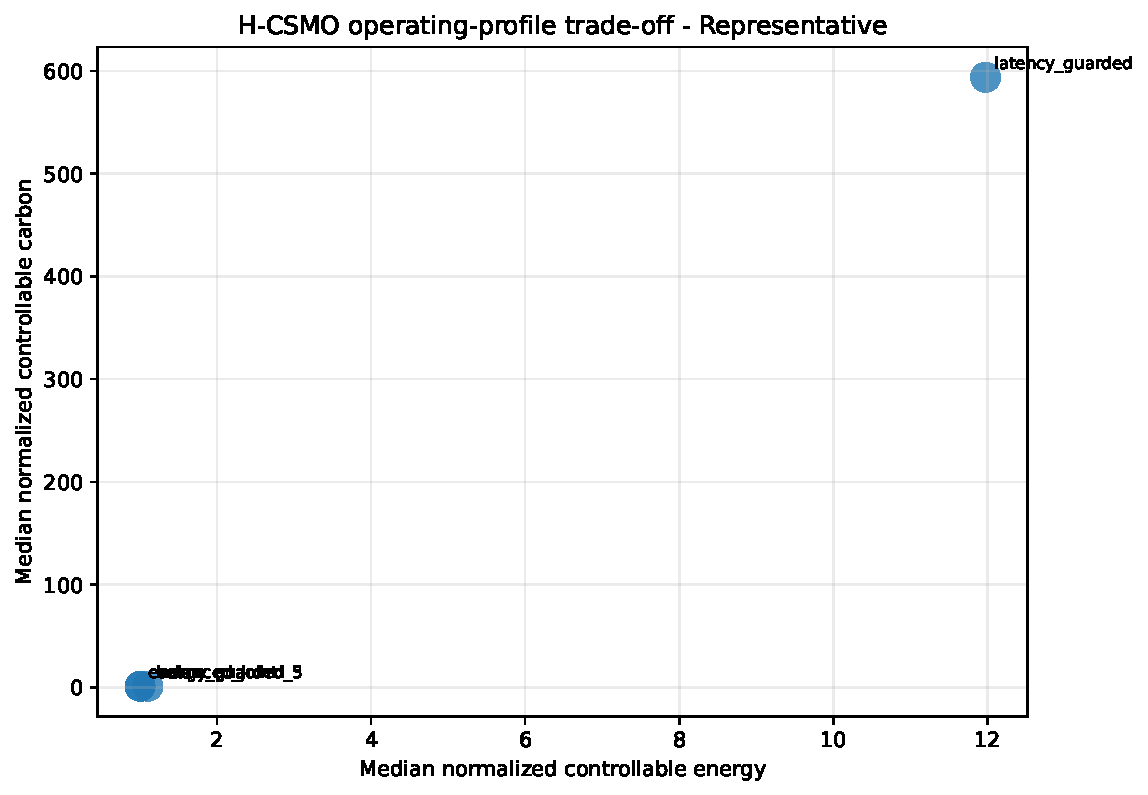
\includegraphics[width=\linewidth]{fig17_profile_tradeoff_representative.pdf}\caption{Representative.}\end{subfigure}\hfill
\begin{subfigure}{0.49\textwidth}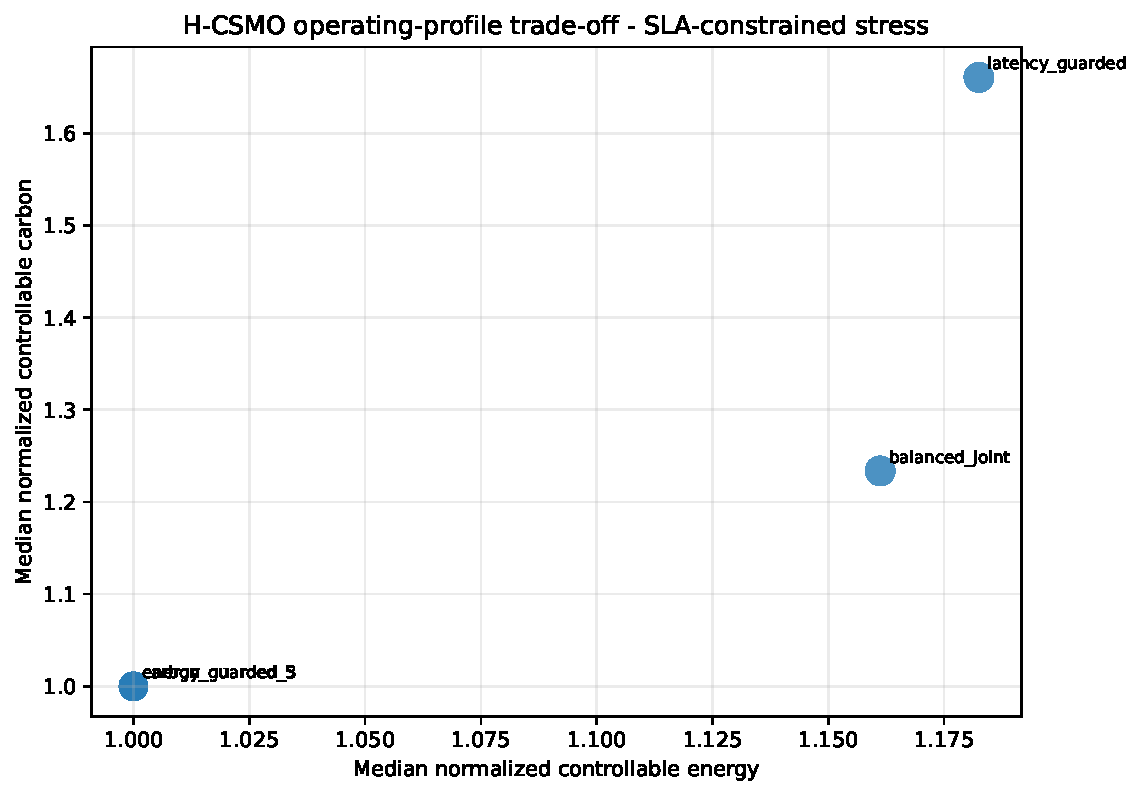
\includegraphics[width=\linewidth]{fig17_profile_tradeoff_sla_stress.pdf}\caption{SLA stress.}\end{subfigure}
\caption{Median operating-profile trade-offs produced by \method.}\label{fig:profiles-appendix}
\end{figure*}
% ---- END sections/10_appendix.tex ----

\section*{Funding}
No funding was received for this work.

\section*{Data and artifact availability}
The experiments use trace-derived scenarios from the Google 2011 cluster workload and Alibaba Cluster Trace v2017. The frozen scenario files, run manifests, per-run decision vectors and schedules, aggregate statistical tables, and figure-generation artifacts used for the reported results are available from the corresponding author on reasonable request.

\bibliographystyle{elsarticle-num}
\bibliography{references}

\end{document}
